\documentclass[sigconf,anonymous]{acmart}

\makeatletter
\global\@ACM@balancefalse
\makeatother
\raggedbottom
\setlength{\emergencystretch}{2em}
\settopmatter{printacmref=true}
\renewcommand\footnotetextcopyrightpermission[1]{}

\acmConference[Preprint]{Manuscript}{2026}{}
\acmYear{2026}
\copyrightyear{2026}
\acmDOI{}
\acmISBN{}

\title{Lag-Aware Self-Supervised Dynamic Graph Structure Discovery for Multivariate Time Series}

\author{Anonymous Authors}
\affiliation{%
  \institution{Anonymous Institution}
  \city{Anonymous City}
  \country{Anonymous Country}}
\email{anonymous@example.com}

\begin{document}

\begin{abstract}
Directed, lag-aware structure discovery from multivariate time series underpins interpretable temporal modeling, yet edge labels and regime annotations are rarely available.
We study label-free recovery of auditable lagged directed graphs when the active graph changes across latent regimes.
We develop STCG, which scores sparse lagged reconstruction inside sliding windows, clusters window-level score tensors at a supplied state count under a label-free acceptance gate, and aggregates per-state graphs into one lagged score tensor.
On the original switching-regime panel over twenty shared seeds, STCG-v1 and the annealed regime specialist Regime-PCMCI have statistically indistinguishable edge recovery (Edge AUC $0.812$ versus $0.816$, two-sided paired $p=0.668$), without establishing equivalence, while matched exclusive timing places the specialist at $5.6\times10^{3}$ times STCG-v1's wall-clock cost. STCG-v1 uses a fixed two-state candidate with a one-state fallback and no annealed search, and significantly outperforms thirteen other reference methods, including windowed VAR-Lasso, neural-Granger cMLP, DYNOTEARS, PCMCI$^+$, and PCMCI-ParCorr; off the switching setting it beats the degraded specialist on every metric while global methods remain strongest.
A preregistered stress extension on fresh seeds bounds this tie: with a supplied regime count, Regime-PCMCI is significantly stronger under fast regime switching and longer sequences, so parity holds at the original operating point rather than across the stress grid. A twenty-partition score ensemble further improves switching Edge AUC to $0.815$ and wins 190 of 260 stress fits.
On selected labeled real transition segments, all compared methods receive the same specified regime count and STCG-v1 obtains positive alignment; additional forward tests at fixed time origins do not establish consistent utility over simpler sensor or graph-feature classifiers.
The claim is deliberately bounded: global methods remain stronger on stationary and strongly nonlinear systems, latent-state recovery is variable across seeds, and real-data forecasting with graph-derived features is diagnostic rather than state of the art.
\end{abstract}

\begin{CCSXML}
<ccs2012>
   <concept>
       <concept_id>10002951.10003227.10003236</concept_id>
       <concept_desc>Information systems~Data mining</concept_desc>
       <concept_significance>500</concept_significance>
   </concept>
   <concept>
       <concept_id>10010147.10010257.10010258.10010261</concept_id>
       <concept_desc>Computing methodologies~Machine learning approaches</concept_desc>
       <concept_significance>500</concept_significance>
   </concept>
</ccs2012>
\end{CCSXML}

\ccsdesc[500]{Information systems~Data mining}
\ccsdesc[500]{Computing methodologies~Machine learning approaches}

\keywords{dynamic graph learning, self-supervised learning, temporal causal discovery, multivariate time series}

\maketitle

\section{Introduction}

Many multivariate time series are generated by sparse lagged interactions, but the dependency graph itself is rarely observed.
Forecasting models can exploit such dependencies implicitly, yet the learned representation is difficult to audit as a directed, lag-aware graph: an attention weight or a hidden state is not a statement that node $i$ at lag $\ell$ drives node $j$.
This creates a gap between predictive temporal modeling and interpretable structure discovery.

We study the label-free version of the problem: only node time series are observed, no edge labels or regime annotations are available, and the active graph may change across latent regimes.
The goal is an auditable artifact---a sparse set of directed lagged edges together with the latent regimes in which they are active---rather than another opaque predictor.
The central question is whether reconstruction-derived temporal signals can recover such structure under regime change, and at what cost relative to methods designed for exactly that setting.

Our answer is deliberately scoped.
On switching-regime synthetic systems, STCG-v1 has an edge-recovery estimate close to Regime-PCMCI~\cite{saggioro2020regime}, the strongest regime-aware specialist (Edge AUC $0.812$ versus $0.816$ over twenty shared seeds, two-sided paired $t$-test $p=0.668$). STCG-v1 tests a fixed two-state partition against a one-state fallback, while Regime-PCMCI uses a two-regime prior and annealed mixed-integer search; neither comparison establishes recovery without a regime-count setting. A dedicated exclusive-timing study measures the specialist at $5.6\times10^{3}$ times STCG-v1's wall-clock cost on this configuration.
On the same benchmark it significantly outperforms windowed VAR-Lasso, neural-Granger cMLP~\cite{tank2021neural}, DYNOTEARS~\cite{pamfil2020dynotears}, PCMCI$^+$~\cite{runge2020pcmciplus}, and PCMCI-ParCorr~\cite{runge2019detecting}.
The boundaries are explicit: on stationary and strongly nonlinear systems, global methods such as VAR-Lasso and cMLP remain stronger while the specialist degrades below STCG-v1 on every metric, and latent-state recovery is variable across seeds. A preregistered stress extension on fresh generator seeds further bounds the central tie: with a supplied regime count, Regime-PCMCI is significantly stronger under fast switching and on longer sequences, so the tie is an operating-point result.
On regime-labeled real sensor data with the same regime-count information given to all methods, STCG-v1 obtains positive regime alignment on every contiguous transition segment we tested, including cases where Regime-PCMCI collapses to a single regime or its annealing fails to converge; block-concatenated data without temporal contiguity still favors the specialist.
Real-data forecasting with graph-derived features is treated as a diagnostic probe, not as a state-of-the-art claim.

This paper makes three contributions.
First, we formalize lag-aware dynamic graph recovery without edge or per-window regime supervision and instantiate it with latent graph-state aggregation: window-level scores are clustered using a supplied state count and an unsupervised acceptance gate, and per-state aggregation denoises the local estimates.
Second, we evaluate against modern structure-recovery baselines, including Regime-PCMCI, finding close point estimates without a significant two-sided difference, together with significant wins over thirteen other reference methods under paired tests; a variance-reduced score ensemble raises switching Edge AUC to $0.815$ and wins 190 of 260 stress fits; a preregistered stress extension on new seeds replicates the tie at the original operating point and reports where it breaks, and a dedicated timing study supplies the previously missing matched cost comparison. We disclose the cMLP pilot-seed overlap and report a sensitivity analysis excluding those seeds.
Third, on real labeled sensor data we contrast descriptive regime alignment with forward diagnosis at prespecified time origins, separating operating-condition association from evidence of practical utility.

\section{Related Work}

Classical temporal discovery begins with Granger-style predictive tests, which ask whether lagged values of one variable improve prediction of another~\cite{granger1969investigating}.
Constraint-based methods instead search over conditional-independence tests: PC-style time-series adaptations, the PCMCI framework for large autocorrelated systems~\cite{runge2019detecting}, its contemporaneous extension PCMCI$^+$~\cite{runge2020pcmciplus}, and LPCMCI, which raises recall under latent confounding~\cite{gerhardus2020lpcmci}.
These methods return auditable lagged graphs and are strong stationary references, but they typically fit one fixed conditional-dependence structure over a series (or over a given regime partition) rather than learning latent dynamic graph states.
PCMCI-ParCorr and PCMCI$^+$ therefore appear as baselines in our synthetic recovery loop.

A second line treats the dependence structure itself as switching across regimes.
In econometrics, Markov-switching models condition autoregressive behavior on a hidden discrete state~\cite{hamilton1989new}. A joint switching VAR uses one shared state chain across its vector equations; an independently fitted regression with autoregressive errors is a different model.
CD-NOD exploits distribution shift as a signal, detecting changing causal mechanisms and orienting edges from heterogeneous or nonstationary data~\cite{huang2020cdnod}.
More recently, SPACETIME~\cite{mameche2025spacetime} uses minimum-description-length scoring to jointly discover temporal graphs, changepoints, and invariant mechanisms across multiple contexts; PCMCI$_\Omega$~\cite{gao2023pcmciomega} targets periodically recurring mechanisms in semi-stationary series, with identification guarantees for discrete-valued series under its stated assumptions.
These are relevant alternatives: STCG supplies neither SPACETIME's consistency result nor PCMCI$_\Omega$'s conditional identification guarantee.
Closest to our setting, Regime-PCMCI couples PCMCI with a persistent latent regime variable and jointly optimizes regime assignments and per-regime graphs through an annealed mixed-integer procedure~\cite{saggioro2020regime}; it also appears as a baseline.
STCG shares the premise that lagged dependencies are regime-dependent, but replaces the annealed mixed-integer search with clustering of lag-aware window scores at a supplied state count, a label-free partition-acceptance gate, and per-state aggregation of scores that are already computed.
Its additional operations are clustering and aggregation; a dedicated matched-timing study (Section~\ref{sec:exp-specialist-stress}) measures the specialist at $5.6\times10^{3}$ times STCG-v1's wall-clock cost on the base switching configuration.

A third line is score-based continuous optimization.
NOTEARS casts DAG learning as a differentiable objective with a smooth acyclicity constraint~\cite{zheng2018dags}; DYNOTEARS extends it to dynamic Bayesian networks with intra- and inter-slice edges~\cite{pamfil2020dynotears}, and NTS-NOTEARS learns nonparametric temporal DAGs with convolutional parent models and prior-knowledge constraints~\cite{sun2023ntsnotears}; DYNOTEARS is among our baselines.
These methods estimate one global dynamic graph under acyclicity machinery.
Because STCG scores only directed lagged relations $i_{t-\ell}\rightarrow j_t$, temporal ordering already resolves orientation, so no acyclicity constraint is needed; the distinct problem we address is how noisy window-level lagged scores should be aggregated when the active graph changes.

Neural Granger methods fit sparse-input predictors whose weights expose directed dependencies: component-wise MLPs and LSTMs~\cite{tank2021neural}, self-explaining networks that additionally expose interaction signs (GVAR)~\cite{marcinkevics2021gvar}, attention-based temporal convolutions with a causal-validation step (TCDF)~\cite{nauta2019tcdf}, and additive vector autoregression with separable source-wise contributions (NAVAR)~\cite{bussmann2021navar}; the component-wise MLP is among our new baselines.
These approaches are reconstruction-driven and label-free, but should not all be described as static graph estimators: GVAR explicitly exposes time-varying generalized coefficients and effect signs.
STCG's narrower distinction is discrete clustering and aggregation of precomputed window scores; it does not provide those signed nonlinear mechanism explanations.

Our empirical panel prioritizes Regime-PCMCI for latent regime recovery, cMLP for sparse neural prediction, DYNOTEARS for continuous graph optimization, and PCMCI$^+$ for constraint-based discovery. The historical switching-regression control is explicitly distinguished from a joint switching VAR below.
The other neural models and CD-NOD, SPACETIME, and PCMCI$_\Omega$ are discussed but not benchmarked; a single-series adaptation is conceivable for SPACETIME, and PCMCI$_\Omega$ is especially relevant to the periodic difficulty sweep.
Their absence limits empirical coverage, so the results establish comparisons with the implemented panel rather than superiority over all nonstationary discovery methods.

Finally, graph-based forecasters such as STGCN~\cite{yu2018spatio}, Graph WaveNet~\cite{wu2019graphwavenet}, and MTGNN~\cite{wu2020connecting}, and sequence forecasters such as Informer~\cite{zhou2021informer}, optimize prediction.
Recent graph models address changing dependence more directly: MSGNet~\cite{cai2024msgnet} combines frequency-based scales with adaptive graph convolution, whereas TimeFilter~\cite{hu2025timefilter} filters spatial--temporal links separately for each patch.
STCG clusters window-level lagged scores; these forecasters instead adapt dependence representations for predictive loss.
They could inform forecasting comparisons or an explicitly defined graph-extraction study, but their native outputs do not specify the same lag--source--target score tensor used by our recovery protocol.
We have not implemented or validated such an extraction mapping and make no superiority claim over these models; the real forecasting, state-diagnosis, and transition-warning tasks remain diagnostic probes.

\section{Problem Formulation}

Given multivariate observations $X_{1:T} \in \mathbb{R}^{T \times N}$, the goal is to learn latent graphs whose edges can be directed and associated with a discrete lag.
No observed edge labels are used during training.
Evaluation on synthetic data compares recovered edges and lags against known ground truth.
For a maximum lag $L$, the recovered score tensor $S \in \mathbb{R}_{\geq 0}^{L \times N \times N}$ uses $S_{\ell i j}$ to score the directed relation $i_{t-\ell}\rightarrow j_t$.
Self-edges are excluded.

\section{Method}

\subsection{Lag-Aware Window Scoring}

For each ordered pair $(i,j)$ and lag $\ell \in \{1,\ldots,L\}$, the method estimates a nonnegative score $s_{ij\ell,w}$ inside window $w$.
The current implementation uses sparse lagged reconstruction as the base self-supervised signal: a lagged design matrix predicts each target node from past source-node values, and coefficient magnitudes become candidate edge scores.
Self-edges are masked.
For window $w=[a,b)$ and target node $j$, define a lagged design matrix $Z_w$ with columns $X_{t-\ell,i}$ and target vector $y_{w,j}=X_{t,j}$.
STCG-v1 fits
\[
\hat{\beta}_{w,j}
= \arg\min_{\beta}
\|y_{w,j}-Z_w\beta\|_2^2 + \lambda \|\beta\|_1,
\]
and maps coefficients to scores by $S_{w,\ell i j}=|\hat{\beta}_{w,j,\ell i}|$.
The coefficient estimator is intentionally close to a dynamic VAR-Lasso baseline.
The distinguishing step is what happens after local scoring: instead of treating each window independently or averaging all windows, STCG-v1 treats window-level score tensors as observations of latent graph regimes.

\subsection{Latent Graph-State Aggregation}

Independent window estimates are noisy, and max aggregation alone can overfit window-specific fluctuations.
STCG-v1 therefore clusters windows using flattened non-self lagged edge-score features.
For each inferred graph state, it aggregates member-window scores, then combines state-level graphs by a max operator to recover edges that are active in at least one regime.
The clustering uses only reconstruction-derived score features, not synthetic edge labels or regime labels.
Let $z_w=\mathrm{vec}_{i\neq j}(S_w)$ be the non-self edge-score feature for window $w$.
K-means assigns a latent state $c_w \in \{1,\ldots,K\}$.
The main scorer receives a candidate state count and decides whether to accept its partition; separate diagnostic scripts can compare several candidate counts, as distinguished in Section~\ref{sec:method-variants}.
Each state graph is
\[
G_k = \mathrm{Agg}\{S_w: c_w=k\},
\]
where the default aggregator is the element-wise mean.
The final score tensor is
\[
S_{\ell i j} = \max_k G_{k,\ell i j}.
\]

\subsection{Design Assumptions, Rationale, and Variants}
\label{sec:method-design}

\subsubsection{Workload Assumptions and Scope}
\label{sec:method-assumptions}

STCG is built for a specific workload, and its assumptions should be checked before applying it:
\begin{itemize}
\item \emph{Multivariate series of moderate dimension.} Each window must support a per-target sparse lagged regression, so window lengths should be comfortably larger than the number of candidate lagged features per target; our synthetic suites use $N{=}8$ nodes, $T{=}1000$ timesteps, and $L{=}3$.
\item \emph{Piecewise-stationary regimes.} The dependency graph is assumed fixed within a regime and to change at switch points, with regimes persisting longer than one window; windows that mix two regimes are the main failure mode and are quantified by the switch-difficulty sweep in Section~\ref{sec:analysis}.
\item \emph{Sparse, lagged edges.} Cross-node influences are assumed sparse and strictly lagged ($\ell \geq 1$), so temporal ordering resolves edge orientation and no acyclicity machinery is needed.
\item \emph{Unsupervised assignments with a supplied state count.} The scorer uses no edge labels or per-window regime labels, but receives a candidate count $K_0$. The main synthetic suite fixes $K_0{=}2$; the real segment comparison supplies the same annotated count to all methods. These experiments do not establish automatic recovery of an unknown regime count.
\end{itemize}
Two settings argue \emph{against} STCG.
If the system is stationary, a single global fit uses all samples at once and is stronger: global VAR-Lasso and PCMCI variants outperform STCG-v1 on our stationary suite.
If dynamics are strongly nonlinear and smooth, neural-Granger predictors such as cMLP~\cite{tank2021neural} model them directly and outperform windowed linear scores.
STCG targets the middle ground: locally near-linear, sparsely coupled, and switching.

\subsubsection{Design Rationale: Windowed Scores as Observations of Latent Regimes}
\label{sec:method-rationale}

The regime-switching literature models a temporal series as a mixture of local linear dynamics indexed by a latent discrete state, from Markov-switching autoregressions~\cite{hamilton1989new} to the persistent regime variable of Regime-PCMCI~\cite{saggioro2020regime}.
STCG keeps that statistical picture but splits the estimation differently.
A windowed sparse regression yields a \emph{local} estimate of the active lagged graph: regularized and noisy, because each window sees few samples.
If regimes persist across many windows, their local scores provide repeated noisy views of similar dependencies; clustering offers a proxy for the state sequence, and averaging pools those views without fitting an explicit transition model.
This is a statistical rationale, not a recovery guarantee: overlapping windows have correlated errors, coefficient magnitudes are biased by regularization, and incorrect clusters can average different mechanisms.
The cross-state max then reassembles the union graph: an edge that is strong in any single regime survives aggregation.
This avoids jointly annealing regime assignments and per-regime graphs~\cite{saggioro2020regime}: everything after window scoring is clustering and averaging of quantities already computed.

\subsubsection{Partition Gate, Diagnostic State-Count Selection, and Variants}
\label{sec:method-variants}

Two prototypes exist.
STCG-v0 trains differentiable lagged gates from temporal reconstruction alone; it does not outperform the best dynamic VAR baseline and serves only as a reference point.
STCG-v1 keeps the reconstruction signal but adds latent graph-state consistency and is the variant evaluated throughout.
An optional state-contrast term, which up-weights edges specific to one state, was tested and removed from the default because it slightly reduced switching-regime recovery (Table~\ref{tab:state-ablation}).
STCG-v1 should therefore not be read as dynamic VAR followed by a post-hoc clustering plot: state inference feeds back into the returned scores, and the no-state ablation in Table~\ref{tab:state-ablation} collapses the method to exactly the windowed baseline.

The main scorer fits one K-means partition at the supplied $K_0$ (capped by the number of windows), rather than searching a candidate set. Its automatic gate accepts this partition on either of two paths.
The primary path accepts an inertia improvement of at least $0.12$ over one state. This is a heuristic separation criterion, not a calibrated test that distinguishes regime change from noise.
The fallback path accepts a weaker partition when three conditions hold jointly: an inertia improvement of at least $0.04$; adjusted temporal coherence of at least $0.55$, favoring repeated assignments beyond their frequency-based expectation; and a minimum state share of $0.10$, discouraging small clusters on this path.
If no partition passes either path, STCG-v1 falls back to a single state and reduces gracefully to its windowed scorer.

Separate real-data diagnostic and warning scripts, not the main synthetic scorer, can sweep a candidate set $\mathcal{K}$ of state counts. In these diagnostics each candidate is scored by
\[
q_K = \frac{\Delta_K \tau_K b_K}{\log_2(K+1)},
\]
where $\Delta_K$ is the score-clustering improvement over one state, $\tau_K$ is adjusted temporal coherence, and $b_K=\min(1,K\pi_{\min})$ penalizes tiny states with minimum state fraction $\pi_{\min}$; the logarithmic denominator prices parsimony, so each additional state must pay for itself in improvement and coherence.
For the Hydraulic transition-warning ablation, we also test a transition-oriented score
\[
q^{\mathrm{warn}}_K =
\frac{\Delta_K b_K(1+\rho_K)/2}{\log_2(K+1)}, \quad
\rho_K = 1-\min(1,\tau_K),
\]
which keeps the balance and parsimony terms but stops rejecting low-coherence partitions, on the argument that windows near regime changes are precisely the warning-relevant ones.
Candidates failing the diagnostic improvement/share screens (and the stable score's coherence screen) receive zero score.
Positive scores are ranked by score, then coherence, then smaller $K$; if none is positive, the corrected selector returns the actually fitted $K{=}1$ candidate.
The historical tie-break could return multiple states even when every score was zero; legacy behavior is retained only for reproducing that diagnostic, and the correction does not change comparisons among positive-score candidates.

\paragraph{Score-space ensemble (STCG-v1e).}
With few windows, the K-means partition is unstable: a different initialization can move a non-trivial share of the aggregation variance into the returned graph.
STCG-v1e therefore averages the aggregated score tensors produced by $B$ K-means partitions (the primary $n_{\mathrm{init}}{=}10$ solution plus $B-1$ restarts),
\[
S^{\mathrm{ens}}_{\ell i j}=\frac{1}{B}\sum_{b=1}^{B}S^{(b)}_{\ell i j},
\]
leaving the acceptance gate unchanged; when the gate rejects the candidate partition, the ensemble returns the one-state scores unchanged.
Averaging in score space reduces partition variance without using labels or changing the state count; $B{=}1$ reproduces STCG-v1 exactly.
We use $B{=}20$ throughout. At the main panel's six-window operating point this adds about $0.1$~s per fit, roughly $1.7\times$ the window-scoring pass, which is still negligible against the specialist's joint search but is not free.

\subsubsection{Heuristic Knobs and Their Empirical Isolation}
\label{sec:method-knobs}

Table~\ref{tab:knob-map} maps each heuristic choice to its role and to the evidence that isolates it.
The state-aggregation mechanism and the removed state-contrast term are isolated by ablation (Table~\ref{tab:state-ablation}); the gate thresholds, aggregators, state features, and window size are swept one factor at a time (Table~\ref{tab:knob-ablation}, Section~\ref{sec:analysis}); and the interaction of window size with switch frequency is covered by the switch-difficulty sweep (Section~\ref{sec:analysis}).
The original knob sweep never changes the accepted partition on the default switching benchmark. A separate eight-condition stress test and controlled score-tensor fixtures exercise acceptance, rejection, and fallback and isolate the selector's balance, coherence, and parsimony factors (Section~\ref{sec:gate-stress}). These diagnose each component's role, not optimality of its numerical threshold or functional form; base-scorer strength is also not independently validated on the synthetic suite.

\begin{table}[t]
\caption{Design knobs, their roles, and the evidence isolating each. ``Design'' marks choices currently justified by argument only, with no dedicated ablation yet.}
\label{tab:knob-map}
\centering
\small
{\sloppy
\setlength{\tabcolsep}{4pt}\begin{tabular}{p{0.22\linewidth}p{0.28\linewidth}p{0.38\linewidth}}
\toprule
Knob & Role & Isolated by \\
\midrule
Window size $h$, stride $r$ & Local estimation granularity; trades locality against per-window sample count & Window-size sweep (Table~\ref{tab:knob-ablation}); sequence-length and switch-difficulty sweeps (Section~\ref{sec:analysis}) \\
Base scorer: per-window VAR-Lasso strength $\lambda$ & Converts local dynamics to sparse lagged edge scores & Design: matches the DynVAR-Lasso baseline so Table~\ref{tab:state-ablation} isolates state aggregation; $\lambda$ swept only in real-data mask sweeps (Section~\ref{sec:experiments}) \\
Non-self score features $z_w$ & State representation; tests the effect of retaining self-lag information & Table~\ref{tab:knob-ablation}: small edge-score changes but different state assignments \\
Within-state mean, cross-state max & Denoise within a regime; union of regime-specific edges & Table~\ref{tab:state-ablation} (no-state vs.\ state-only); Table~\ref{tab:knob-ablation} (aggregator variants): sensitivity of mean recovery \\
Auto-gate thresholds $0.12$ / $0.04$ / $0.55$ / $0.10$ & Heuristic acceptance and persistence fallback & Original sweep never binding; new path removals and stationary negative controls (Table~\ref{tab:gate-stress}) expose both utility and false splitting \\
State-contrast term & Up-weights state-specific edges & Table~\ref{tab:state-ablation}: negative ablation, removed from the default \\
$q_K$ parsimony $\log_2(K{+}1)$; $q^{\mathrm{warn}}_K$ & Discourages extra states; warning-oriented ranking & Factor removals on generated data and controlled hierarchy fixtures (Section~\ref{sec:gate-stress}); functional form remains heuristic \\
\bottomrule
\end{tabular}}
\Description{Knob mapping table linking each heuristic design choice to its role and to the ablation, sweep, or design argument that justifies it.}
\end{table}

\subsection{Algorithm}

Figure~\ref{alg:stcg-v1} summarizes the implemented STCG-v1 pipeline end to end.

\begin{figure}[t]
\centering
\small
\begin{tabular}{p{0.96\linewidth}}
\toprule
\textbf{Algorithm 1: STCG-v1 graph-state scoring} \\
\textbf{Input:} time series $X_{1:T}$, maximum lag $L$, window size $h$, stride $r$, supplied state count $K_0$ and gate thresholds. \\
1. Form overlapping windows $w_1,\ldots,w_M$ using size $h$ and stride $r$. \\
2. For each window and target node, fit sparse lagged reconstruction and store non-self score tensor $S_w$. \\
3. Flatten each $S_w$ into a non-self graph feature $z_w$. \\
4. Standardize $\{z_w\}$ across windows and fit K-means at $K=\min(K_0,M)$. Compute inertia improvement, temporal coherence, and minimum state share. \\
5. Accept the partition if either gate path passes; otherwise return the plain window-aggregated scores. No search across candidate counts occurs in this scorer. \\
6. Aggregate window score tensors within each selected state to obtain $G_k$. \\
7. Return $S_{\ell i j}=\max_k G_{k,\ell i j}$ for structure recovery, graph-prior forecasting, or warning probes. \\
\bottomrule
\end{tabular}
\caption{Implemented STCG-v1 scorer. Edge labels and per-window regime labels are not used in steps 1--7; the state count is supplied. Separate diagnostic scripts implement multi-$K$ selection. The real segment comparison supplies annotated $K$ and sets the acceptance threshold to zero.}
\Description{Pseudocode listing the seven implemented STCG-v1 steps from sliding-window lagged reconstruction through graph-state clustering and state-level score aggregation.}
\label{alg:stcg-v1}
\end{figure}

\subsection{Graph-Guided Forecasting Probe}

For real-data probing, graph scores are converted either to a hard non-self feature mask or to a soft ridge prior.
The hard probe keeps the top-scoring non-self lagged sources for each target.
The soft probe keeps all lagged features and changes only the ridge penalty.
Given a target-specific feature weight $w_{mj}>0$, it fits
\[
\hat{\beta}_j
= \arg\min_{\beta}
\|y_j-Z\beta\|_2^2 + \alpha \sum_m \frac{\beta_m^2}{w_{mj}}.
\]
Weights are normalized from the score tensor per target, with self-lag features assigned unit weight.
Thus a high graph score weakens shrinkage for that lagged source, while low-score features remain available rather than being deleted.

\subsection{Real-Data Diagnostic Protocols}

The predictive real-data probes use chronological splits.
Graph scores, scalers, masks, and ridge priors are fit only on the training segment before one-step forecasting is evaluated on future samples. Full-series state alignment and capped-segment regime recovery are retrospective descriptive analyses rather than held-out prediction.
The historical random-window state-label diagnostics fit graph states on the full series and use overlapping windows, so their balanced accuracy and macro F1 are optimistic descriptive diagnostics. The forward-only variant fits states and label mappings on chronological training windows and excludes windows crossing the split.
For Hydraulic transition warnings, each example uses only a lookback of past cycles and the target is whether the audited label changes within the next horizon.
Classifiers are trained on the earliest segment, thresholds and optional STCG warning configurations are selected on the following chronological validation segment, and final AP/F1/ROC AUC are reported once on the final test segment. Examples whose future target horizon reaches the next segment are purged before fitting or validation selection.

\section{Experiments}
\label{sec:experiments}

\subsection{Synthetic Setup}
\label{sec:exp-synthetic-setup}

The primary experiments use three generators with known directed lagged edges: stationary VAR, nonlinear VAR, and a switching-regime VAR whose active graph changes at a midpoint regime switch.
The main synthetic recovery tables use twenty shared seeds with $N{=}8$ nodes, $T{=}1000$ timesteps, maximum lag $L{=}3$, window size $300$, and stride $150$, matching the workload assumptions of Section~\ref{sec:method-assumptions}. The switch-difficulty sweep uses ten seeds, the state diagnostics five, and robustness and knob sweeps twenty; sweep axes can override these defaults.
Metrics are Edge AUC over lagged directed edges, Pair AUC after collapsing lags, Precision@K at the number of true edges, Structural Hamming Distance (SHD), and lag recovery accuracy for correctly recovered directed pairs.
Paired tests compare methods on the same seeds, with bootstrap confidence intervals and one-sided paired $t$-tests and Wilcoxon tests for superiority. We additionally report two-sided tests for differences from Regime-PCMCI. No equivalence or non-inferiority margin was specified, so nonsignificance does not establish equivalence.

Fourteen reference methods span the discovery families surveyed above; a separately identified legacy control remains in the historical table for traceability.
\emph{Global stationary} methods fit one structure on the full series: lagged correlation (LagCorr), VAR-Ridge, VAR-Lasso, Granger-F tests~\cite{granger1969investigating}, PCMCI with ParCorr tests~\cite{runge2019detecting}, and its contemporaneous extension PCMCI$^+$~\cite{runge2020pcmciplus}.
\emph{Regime-aware} discovery is represented by Regime-PCMCI~\cite{saggioro2020regime}, given a two-regime prior that equals the true count on the switching generator. STCG-v1 also receives a fixed two-state candidate on all three generators, with its default one-state fallback enabled.
The legacy \emph{MSAR-X} control fits independent switching regressions with autoregressive residuals. It was previously mislabeled MSVAR: residual autoregression introduces coefficient interactions and cross-lags beyond the requested order, so its exogenous-coefficient scores are not direct VAR($L$) coefficients. Its aligned posterior average is also not a shared-chain joint fit. We retain its recorded results under the corrected name but exclude it from claims of superiority over joint MSVAR.
A post-audit corrective comparison supplies the missing joint model: a shared-chain Gaussian MS-VAR(3) with direct VAR means and full regime covariance, frozen before fitting and evaluated on the base switching configuration over fresh seeds 100--119 with ten starts per seed and a 200-iteration EM budget.
All twenty fits converge, and STCG-v1 is statistically tied with the joint MSVAR on this condition (Edge AUC $0.827$ versus $0.817$; difference $+0.0109$, 95\% CI $[-0.0174, 0.0463]$; two-sided $p_t=0.527$, $p_W=0.430$).
This single-condition corrective result replaces the withdrawn superiority claim over joint MSVAR; it does not extend across the stress grid of Section~\ref{sec:exp-specialist-stress}.
\emph{Score-based} search is represented by DYNOTEARS~\cite{pamfil2020dynotears}, which fits one global dynamic Bayesian network.
\emph{Neural Granger} is represented by the component-wise MLP (cMLP)~\cite{tank2021neural}.
Its hyperparameters were chosen on pilot seeds 0--4 of these same generators, which overlap the twenty-seed descriptive table. A retrospective sensitivity analysis excludes those seeds and uses common remaining seeds for all sixteen methods: 5--19 on stationary and switching VAR, and the same set without seed 18 on nonlinear VAR because that RPCMCI fit failed. This is not a newly collected independent confirmation set.
\emph{Windowed dynamic} baselines (DynVAR-Ridge, DynVAR-Lasso, DynGranger-F) apply the same sliding-window scoring as STCG-v1 but aggregate windows by a plain max.
Random scores and STCG-v0, the gate-only prototype, complete the roster as reference points.

\subsection{Synthetic Recovery Results}
\label{sec:exp-synthetic-results}

\begin{table*}[t]
\caption{Descriptive structure recovery across three generators over twenty shared seeds (mean $\pm$ std), including five cMLP pilot seeds. Higher is better except for SHD; bold marks the best mean. MSAR-X is the corrected name of the legacy switching-regression control, not joint MSVAR. Fit time is tracked for MSAR-X, Regime-PCMCI, cMLP, and DYNOTEARS, but not STCG; Section~\ref{sec:exp-specialist-stress} reports the dedicated matched-timing study that closes this gap. Regime-PCMCI on nonlinear VAR has $n{=}19$: seed 18 did not converge. The artifact includes post-pilot comparisons on identical common seeds.}
\label{tab:all-methods}
\centering
\footnotesize
\setlength{\tabcolsep}{4pt}
\begin{tabular}{llrrrrrr}
\toprule
Generator & Method & Edge AUC & Pair AUC & P@K & SHD & Lag Acc & Fit Time (s) \\
\midrule
nonlinear\_var & DYNOTEARS & 0.946 $\pm$ 0.069 & 0.965 $\pm$ 0.049 & 0.881 $\pm$ 0.114 & 7.8 $\pm$ 8.5 & 0.933 $\pm$ 0.101 & 0.1 \\
nonlinear\_var & DynGranger-F & 0.975 $\pm$ 0.027 & 0.973 $\pm$ 0.025 & 0.878 $\pm$ 0.067 & 7.6 $\pm$ 4.7 & 0.964 $\pm$ 0.049 & n/a \\
nonlinear\_var & DynVAR-Lasso & 0.956 $\pm$ 0.050 & 0.942 $\pm$ 0.047 & 0.820 $\pm$ 0.100 & 11.3 $\pm$ 7.8 & 0.969 $\pm$ 0.057 & n/a \\
nonlinear\_var & DynVAR-Ridge & 0.943 $\pm$ 0.051 & 0.917 $\pm$ 0.062 & 0.767 $\pm$ 0.112 & 14.5 $\pm$ 8.9 & 0.964 $\pm$ 0.048 & n/a \\
nonlinear\_var & Granger-F & 0.981 $\pm$ 0.028 & \textbf{0.985 $\pm$ 0.021} & \textbf{0.925 $\pm$ 0.066} & \textbf{4.8 $\pm$ 4.7} & 0.977 $\pm$ 0.051 & n/a \\
nonlinear\_var & LagCorr & 0.787 $\pm$ 0.090 & 0.786 $\pm$ 0.087 & 0.531 $\pm$ 0.097 & 28.8 $\pm$ 9.9 & 0.733 $\pm$ 0.100 & n/a \\
nonlinear\_var & MSAR-X (legacy) & 0.895 $\pm$ 0.051 & 0.827 $\pm$ 0.075 & 0.627 $\pm$ 0.115 & 22.6 $\pm$ 8.5 & 0.915 $\pm$ 0.049 & 170.7 \\
nonlinear\_var & PCMCI+ & 0.919 $\pm$ 0.052 & 0.944 $\pm$ 0.045 & 0.837 $\pm$ 0.091 & 10.3 $\pm$ 7.6 & 0.901 $\pm$ 0.071 & n/a \\
nonlinear\_var & PCMCI-ParCorr & \textbf{0.984 $\pm$ 0.023} & 0.985 $\pm$ 0.019 & 0.924 $\pm$ 0.064 & 4.9 $\pm$ 4.8 & 0.971 $\pm$ 0.048 & n/a \\
nonlinear\_var & Random & 0.485 $\pm$ 0.060 & 0.483 $\pm$ 0.069 & 0.169 $\pm$ 0.062 & 49.8 $\pm$ 7.5 & 0.424 $\pm$ 0.078 & n/a \\
nonlinear\_var & Regime-PCMCI & 0.767 $\pm$ 0.167 & 0.698 $\pm$ 0.190 & 0.468 $\pm$ 0.260 & 32.6 $\pm$ 18.6 & 0.704 $\pm$ 0.221 & 164.8 \\
nonlinear\_var & STCG-v0 & 0.948 $\pm$ 0.049 & 0.925 $\pm$ 0.059 & 0.781 $\pm$ 0.107 & 13.5 $\pm$ 7.7 & 0.957 $\pm$ 0.059 & n/a \\
nonlinear\_var & STCG-v1 & 0.969 $\pm$ 0.040 & 0.964 $\pm$ 0.033 & 0.860 $\pm$ 0.088 & 8.9 $\pm$ 7.0 & 0.976 $\pm$ 0.049 & n/a \\
nonlinear\_var & VAR-Lasso & 0.978 $\pm$ 0.041 & 0.980 $\pm$ 0.029 & 0.912 $\pm$ 0.088 & 5.7 $\pm$ 6.5 & 0.982 $\pm$ 0.057 & n/a \\
nonlinear\_var & VAR-Ridge & 0.973 $\pm$ 0.037 & 0.969 $\pm$ 0.037 & 0.881 $\pm$ 0.095 & 7.6 $\pm$ 7.1 & 0.982 $\pm$ 0.050 & n/a \\
nonlinear\_var & cMLP & 0.980 $\pm$ 0.032 & 0.974 $\pm$ 0.020 & 0.886 $\pm$ 0.063 & 7.1 $\pm$ 4.8 & \textbf{0.985 $\pm$ 0.049} & 0.6 \\
\midrule
switching\_var & DYNOTEARS & 0.746 $\pm$ 0.037 & 0.795 $\pm$ 0.047 & 0.586 $\pm$ 0.067 & 45.2 $\pm$ 9.2 & 0.697 $\pm$ 0.064 & 0.0 \\
switching\_var & DynGranger-F & 0.797 $\pm$ 0.039 & 0.830 $\pm$ 0.055 & 0.650 $\pm$ 0.044 & 38.1 $\pm$ 5.9 & 0.791 $\pm$ 0.052 & n/a \\
switching\_var & DynVAR-Lasso & 0.798 $\pm$ 0.040 & 0.830 $\pm$ 0.058 & 0.646 $\pm$ 0.047 & 38.6 $\pm$ 6.4 & 0.797 $\pm$ 0.058 & n/a \\
switching\_var & DynVAR-Ridge & 0.796 $\pm$ 0.040 & 0.827 $\pm$ 0.057 & 0.642 $\pm$ 0.047 & 39.0 $\pm$ 6.2 & 0.791 $\pm$ 0.055 & n/a \\
switching\_var & Granger-F & 0.778 $\pm$ 0.046 & 0.806 $\pm$ 0.051 & 0.622 $\pm$ 0.050 & 41.2 $\pm$ 7.0 & 0.770 $\pm$ 0.063 & n/a \\
switching\_var & LagCorr & 0.770 $\pm$ 0.047 & 0.805 $\pm$ 0.045 & 0.617 $\pm$ 0.050 & 41.8 $\pm$ 7.7 & 0.764 $\pm$ 0.060 & n/a \\
switching\_var & MSAR-X (legacy) & 0.613 $\pm$ 0.044 & 0.610 $\pm$ 0.072 & 0.409 $\pm$ 0.053 & 64.2 $\pm$ 6.8 & 0.568 $\pm$ 0.077 & 145.6 \\
switching\_var & PCMCI+ & 0.769 $\pm$ 0.048 & 0.808 $\pm$ 0.048 & 0.618 $\pm$ 0.051 & 41.6 $\pm$ 7.3 & 0.756 $\pm$ 0.060 & n/a \\
switching\_var & PCMCI-ParCorr & 0.779 $\pm$ 0.045 & 0.809 $\pm$ 0.049 & 0.621 $\pm$ 0.044 & 41.3 $\pm$ 6.7 & 0.760 $\pm$ 0.055 & n/a \\
switching\_var & Random & 0.478 $\pm$ 0.053 & 0.472 $\pm$ 0.081 & 0.301 $\pm$ 0.066 & 75.7 $\pm$ 6.8 & 0.465 $\pm$ 0.079 & n/a \\
switching\_var & Regime-PCMCI & \textbf{0.816 $\pm$ 0.036} & 0.832 $\pm$ 0.045 & 0.661 $\pm$ 0.054 & 36.6 $\pm$ 4.9 & \textbf{0.823 $\pm$ 0.058} & 204.7 \\
switching\_var & STCG-v0 & 0.780 $\pm$ 0.042 & 0.790 $\pm$ 0.073 & 0.615 $\pm$ 0.047 & 41.9 $\pm$ 6.6 & 0.777 $\pm$ 0.067 & n/a \\
switching\_var & STCG-v1 & 0.812 $\pm$ 0.047 & \textbf{0.839 $\pm$ 0.058} & \textbf{0.673 $\pm$ 0.059} & \textbf{35.5 $\pm$ 6.5} & 0.811 $\pm$ 0.062 & n/a \\
switching\_var & VAR-Lasso & 0.780 $\pm$ 0.046 & 0.808 $\pm$ 0.052 & 0.625 $\pm$ 0.052 & 40.8 $\pm$ 6.9 & 0.767 $\pm$ 0.062 & n/a \\
switching\_var & VAR-Ridge & 0.779 $\pm$ 0.046 & 0.806 $\pm$ 0.053 & 0.624 $\pm$ 0.053 & 41.0 $\pm$ 7.3 & 0.770 $\pm$ 0.068 & n/a \\
switching\_var & cMLP & 0.780 $\pm$ 0.047 & 0.809 $\pm$ 0.058 & 0.624 $\pm$ 0.048 & 40.9 $\pm$ 6.7 & 0.766 $\pm$ 0.068 & 0.6 \\
\midrule
var & DYNOTEARS & 0.904 $\pm$ 0.034 & 0.912 $\pm$ 0.046 & 0.761 $\pm$ 0.067 & 14.1 $\pm$ 3.4 & 0.854 $\pm$ 0.071 & 0.0 \\
var & DynGranger-F & 0.861 $\pm$ 0.042 & 0.846 $\pm$ 0.059 & 0.639 $\pm$ 0.063 & 21.5 $\pm$ 4.1 & 0.838 $\pm$ 0.072 & n/a \\
var & DynVAR-Lasso & 0.866 $\pm$ 0.041 & 0.849 $\pm$ 0.057 & 0.645 $\pm$ 0.064 & 21.2 $\pm$ 4.2 & 0.847 $\pm$ 0.080 & n/a \\
var & DynVAR-Ridge & 0.862 $\pm$ 0.041 & 0.847 $\pm$ 0.056 & 0.643 $\pm$ 0.061 & 21.3 $\pm$ 4.0 & 0.842 $\pm$ 0.079 & n/a \\
var & Granger-F & 0.920 $\pm$ 0.033 & 0.915 $\pm$ 0.043 & \textbf{0.766 $\pm$ 0.058} & \textbf{13.9 $\pm$ 3.3} & 0.888 $\pm$ 0.063 & n/a \\
var & LagCorr & 0.917 $\pm$ 0.027 & 0.902 $\pm$ 0.034 & 0.735 $\pm$ 0.052 & 15.9 $\pm$ 3.9 & \textbf{0.909 $\pm$ 0.064} & n/a \\
var & MSAR-X (legacy) & 0.743 $\pm$ 0.051 & 0.662 $\pm$ 0.074 & 0.400 $\pm$ 0.095 & 35.7 $\pm$ 6.0 & 0.680 $\pm$ 0.093 & 133.0 \\
var & PCMCI+ & 0.921 $\pm$ 0.027 & 0.912 $\pm$ 0.045 & 0.753 $\pm$ 0.075 & 14.6 $\pm$ 3.8 & 0.905 $\pm$ 0.061 & n/a \\
var & PCMCI-ParCorr & 0.920 $\pm$ 0.035 & 0.915 $\pm$ 0.041 & 0.749 $\pm$ 0.064 & 14.9 $\pm$ 3.6 & 0.873 $\pm$ 0.067 & n/a \\
var & Random & 0.485 $\pm$ 0.060 & 0.483 $\pm$ 0.069 & 0.169 $\pm$ 0.062 & 49.8 $\pm$ 7.5 & 0.424 $\pm$ 0.078 & n/a \\
var & Regime-PCMCI & 0.809 $\pm$ 0.095 & 0.749 $\pm$ 0.116 & 0.514 $\pm$ 0.156 & 29.5 $\pm$ 11.6 & 0.756 $\pm$ 0.147 & 193.9 \\
var & STCG-v0 & 0.847 $\pm$ 0.047 & 0.849 $\pm$ 0.048 & 0.631 $\pm$ 0.064 & 22.1 $\pm$ 4.7 & 0.807 $\pm$ 0.107 & n/a \\
var & STCG-v1 & 0.876 $\pm$ 0.039 & 0.874 $\pm$ 0.049 & 0.665 $\pm$ 0.065 & 19.9 $\pm$ 3.8 & 0.845 $\pm$ 0.081 & n/a \\
var & VAR-Lasso & \textbf{0.924 $\pm$ 0.031} & \textbf{0.916 $\pm$ 0.043} & 0.766 $\pm$ 0.058 & 13.9 $\pm$ 3.3 & 0.890 $\pm$ 0.066 & n/a \\
var & VAR-Ridge & 0.921 $\pm$ 0.033 & 0.915 $\pm$ 0.042 & 0.764 $\pm$ 0.060 & 14.0 $\pm$ 3.4 & 0.887 $\pm$ 0.069 & n/a \\
var & cMLP & 0.918 $\pm$ 0.033 & 0.909 $\pm$ 0.048 & 0.749 $\pm$ 0.068 & 14.8 $\pm$ 3.4 & 0.880 $\pm$ 0.063 & 0.6 \\
\bottomrule
\end{tabular}

\Description{Full synthetic recovery table comparing sixteen methods on stationary, nonlinear, and switching VAR generators by edge AUC, pair AUC, precision at K, structural Hamming distance, lag accuracy, and per-fit seconds.}
\end{table*}

\paragraph{RQ1: does STCG-v1 hold up on switching-regime systems?}
On the switching generator---the setting STCG is built for---Table~\ref{tab:all-methods} shows close point estimates for STCG-v1 and Regime-PCMCI on the primary metric: Edge AUC $0.812$ versus $0.816$ over twenty shared seeds (mean improvement $-0.0031$, 95\% bootstrap CI $[-0.0165, 0.0110]$, one-sided paired $t$-test $p=0.666$, Wilcoxon $p=0.715$; Table~\ref{tab:paired-rpcmci}). Two-sided tests also detect no significant Edge AUC difference ($p_t=0.668$, $p_W=0.596$), but the interval allows a meaningful loss or gain and does not establish equivalence.
The one-sided superiority tests on the remaining metrics are likewise nonsignificant (Pair AUC $p=0.305$, P@K $p=0.149$, SHD $p=0.180$, lag accuracy $p=0.792$); their two-sided results are supplied in the artifact. STCG-v1 attains the best Pair AUC, P@K, and SHD means of all sixteen methods.
Against the thirteen remaining reference methods (excluding the legacy MSAR-X control), every paired Edge AUC test reaches $p \leq 0.0014$ under both the paired $t$ and Wilcoxon tests (Table~\ref{tab:paired-edge-matrix}), including the strongest windowed opponent DynVAR-Lasso ($+0.0143$, $p_t=0.0007$; Table~\ref{tab:paired-switching}) and the stationary constraint-based reference PCMCI-ParCorr ($+0.0334$, $p_t=0.0005$; Table~\ref{tab:paired-pcmci}).
After excluding the cMLP pilot seeds, switching Edge AUC is $0.803$ for STCG-v1 and $0.775$ for cMLP over fifteen common seeds (improvement $+0.0284$, one-sided $p_t=0.0086$, $p_W=0.0051$). The artifact reports all-method common-seed summaries and paired tests for this sensitivity analysis.
The supported conclusion is competitive edge-recovery estimates using score clustering instead of annealed joint search, with state-count information supplied to both approaches.
The frozen stress extension of Section~\ref{sec:exp-specialist-stress} re-tests this conclusion on fresh seeds: the tie replicates at this operating point, but not under fast switching or on longer sequences.

\begin{table}[t]
\caption{Paired STCG-v1 versus Regime-PCMCI tests on switching-regime recovery over twenty seeds. Positive improvement means STCG-v1 is better; for SHD it means fewer errors. $p_t$ and $p_W$ are one-sided superiority tests. None establishes superiority; these tests do not establish equivalence.}
\label{tab:paired-rpcmci}
\centering
\small
\resizebox{\linewidth}{!}{\begin{tabular}{lrrrlrrl}
\toprule
Metric & STCG-v1 & Regime-PCMCI & Improve & 95\% CI & $p_t$ & $p_W$ & W/T/L \\
\midrule
Edge AUC & 0.812 & 0.816 & -0.0031 & [-0.0165, 0.0110] & 0.6659 & 0.7147 & 8/0/12 \\
Pair AUC & 0.839 & 0.832 & 0.0071 & [-0.0184, 0.0339] & 0.3054 & 0.4347 & 9/0/11 \\
P@K & 0.673 & 0.661 & 0.0117 & [-0.0089, 0.0329] & 0.1491 & 0.1429 & 12/2/6 \\
SHD & 35.5 & 36.6 & 1.1 & [-1.1, 3.3] & 0.1803 & 0.2022 & 12/2/6 \\
Lag Acc & 0.811 & 0.823 & -0.0120 & [-0.0388, 0.0167] & 0.7922 & 0.8173 & 6/4/10 \\
\bottomrule
\end{tabular}
}
\Description{Paired synthetic comparison table showing STCG-v1, Regime-PCMCI, mean improvement, bootstrap confidence intervals, paired t-test p-values, Wilcoxon p-values, and win-tie-loss counts on the switching generator.}
\end{table}

\begin{table}[t]
\caption{Paired STCG-v1 Edge AUC against every opponent on switching-regime recovery (twenty shared seeds, sorted by opponent mean). Positive improvement means STCG-v1 is better. All opponents except Regime-PCMCI lose significantly under both tests.}
\label{tab:paired-edge-matrix}
\centering
\small
\resizebox{\linewidth}{!}{\begin{tabular}{lrrrrl}
\toprule
Opponent & Mean & Improv. & 95\% CI & $p_t$ & $p_W$ \\
\midrule
Regime-PCMCI & 0.816 & -0.0031 & [-0.0165, 0.0110] & 0.6659 & 0.7147 \\
DynVAR-Lasso & 0.798 & +0.0143 & [0.0067, 0.0213] & 0.0007 & 0.0014 \\
DynGranger-F & 0.797 & +0.0158 & [0.0080, 0.0230] & 0.0004 & 0.0007 \\
DynVAR-Ridge & 0.796 & +0.0164 & [0.0084, 0.0234] & 0.0003 & 0.0008 \\
cMLP & 0.780 & +0.0322 & [0.0140, 0.0480] & 0.0007 & 0.0004 \\
STCG-v0 & 0.780 & +0.0323 & [0.0195, 0.0451] & $<$1e-4 & 0.0002 \\
VAR-Lasso & 0.780 & +0.0329 & [0.0157, 0.0481] & 0.0004 & 0.0004 \\
PCMCI-ParCorr & 0.779 & +0.0334 & [0.0161, 0.0492] & 0.0005 & 0.0004 \\
VAR-Ridge & 0.779 & +0.0337 & [0.0154, 0.0497] & 0.0006 & 0.0004 \\
Granger-F & 0.778 & +0.0342 & [0.0159, 0.0502] & 0.0005 & 0.0004 \\
LagCorr & 0.770 & +0.0420 & [0.0256, 0.0584] & $<$1e-4 & $<$1e-4 \\
PCMCI$^+$ & 0.769 & +0.0433 & [0.0272, 0.0591] & $<$1e-4 & $<$1e-4 \\
DYNOTEARS & 0.746 & +0.0664 & [0.0532, 0.0802] & $<$1e-4 & $<$1e-4 \\
MSAR-X (legacy) & 0.613 & +0.1996 & [0.1752, 0.2241] & $<$1e-4 & $<$1e-4 \\
Random & 0.478 & +0.3341 & [0.3037, 0.3664] & $<$1e-4 & $<$1e-4 \\
\bottomrule
\end{tabular}
}
\Description{Paired matrix of STCG-v1 edge AUC against fifteen opponents on the switching generator, with mean improvement, bootstrap confidence interval, paired t-test and Wilcoxon p-values.}
\end{table}

\paragraph{RQ2: what happens off the switching setting?}
Global methods that pool all samples remain stronger when the graph never changes.
On stationary VAR, VAR-Lasso ($0.924$), PCMCI$^+$ ($0.921$), PCMCI-ParCorr ($0.920$), and cMLP ($0.918$) all exceed STCG-v1 ($0.876$); on nonlinear VAR, PCMCI-ParCorr ($0.984$), Granger-F ($0.981$), and cMLP ($0.980$) exceed STCG-v1 ($0.969$).
This is the expected cost of windowed estimation, and we report it as a boundary rather than a failure.
The regime specialist degrades far more sharply off its home turf: Regime-PCMCI falls to $0.809$ on stationary VAR and $0.767$ on nonlinear VAR ($n{=}19$), so STCG-v1 beats it there on all five metrics on both generators (paired $p \leq 0.023$ throughout, per-generator paired tables in the artifact).
Windowed linear scoring with state aggregation is therefore more robust than the annealed specialist outside the switching setting, even though single-fit global methods are stronger still.

\paragraph{RQ3: what does regime awareness cost?}
The fit-time column of Table~\ref{tab:all-methods} records costs for four baseline runners.
Regime-PCMCI costs $164.8$--$204.7$ s per fit across the three generators ($204.7$ s on switching), and the legacy MSAR-X control costs $133.0$--$170.7$ s. The latter does not measure joint MSVAR cost. The original synthetic runs did not record matched STCG-v1 end-to-end timings; the dedicated exclusive timing phase of Section~\ref{sec:exp-specialist-stress} fills that gap, measuring a $5575\times$ wall-clock ratio of Regime-PCMCI to STCG-v1 on the base switching configuration while VAR-Lasso and DynVAR-Lasso run faster than STCG-v1 itself. A separate capped real-segment comparison reports measured times under its specified protocol below.
Cheap baselines confirm that low cost alone does not buy switching structure: cMLP ($0.6$ s) and DYNOTEARS ($\leq 0.1$ s) sit $0.03$--$0.07$ Edge AUC below STCG-v1 on the switching generator.

\paragraph{RQ4: does label-free state inference capture the oracle gain?}
An oracle-state diagnostic aggregates window scores by the \emph{true} synthetic regimes, using ground truth only after local scoring.
On the same twenty switching seeds, STCG-v1's inferred-state aggregation nearly matches this upper bound: Edge AUC $0.812$ versus oracle $0.813$ and no-state $0.798$, and P@K $0.673$ versus oracle $0.672$ and no-state $0.646$ (Table~\ref{tab:state-oracle}).
Under the default switching setup, most of the available oracle-state gain is therefore already captured without regime labels; Section~\ref{sec:analysis} examines where the inferred states themselves fall short.

\begin{table}[t]
\caption{Oracle-state diagnostic on twenty-seed switching-regime recovery. The oracle uses true regime labels only after local window scoring and is an upper-bound analysis, not a supervised variant.}
\label{tab:state-oracle}
\centering
\small
\begin{tabular}{lrrrr}
\toprule
Method & Edge AUC & P@K & SHD & Lag Acc. \\
\midrule
DynVAR-Lasso & 0.798 & 0.646 & 38.6 & 0.797 \\
Oracle-state upper bound & 0.813 & 0.672 & 35.6 & 0.800 \\
STCG-v1/inferred-state & 0.812 & 0.673 & 35.5 & 0.811 \\
STCG-v1/no-state & 0.798 & 0.646 & 38.6 & 0.797 \\
\bottomrule
\end{tabular}

\Description{Oracle-state table comparing DynVAR-Lasso, the oracle-state upper bound, STCG-v1 with inferred states, and STCG-v1 without state aggregation by edge AUC, precision at K, structural Hamming distance, and lag accuracy.}
\end{table}

\begin{table}[t]
\caption{Paired STCG-v1 versus DynVAR-Lasso tests on switching-regime recovery. Positive improvement means STCG-v1 is better; for SHD it means fewer errors. $p_t$ is the one-sided paired $t$-test and $p_W$ is the one-sided Wilcoxon signed-rank test.}
\label{tab:paired-switching}
\centering
\small
\resizebox{\linewidth}{!}{\begin{tabular}{lrrrlrrl}
\toprule
Metric & STCG-v1 & DynVAR & Improve & 95\% CI & $p_t$ & $p_W$ & W/T/L \\
\midrule
Edge AUC & 0.812 & 0.798 & 0.0143 & [0.0067, 0.0213] & 0.0007 & 0.0014 & 17/0/3 \\
Pair AUC & 0.839 & 0.830 & 0.0092 & [-0.0081, 0.0272] & 0.1683 & 0.2045 & 11/0/9 \\
P@K & 0.673 & 0.646 & 0.0274 & [0.0150, 0.0403] & 0.0003 & 0.0012 & 14/4/2 \\
SHD & 35.5 & 38.6 & 3.1 & [1.7, 4.6] & 0.0003 & 0.0007 & 14/4/2 \\
Lag Acc & 0.811 & 0.797 & 0.0143 & [-0.0055, 0.0366] & 0.1054 & 0.1896 & 9/6/5 \\
\bottomrule
\end{tabular}
}
\Description{Paired synthetic comparison table showing STCG-v1, DynVAR-Lasso, mean improvement, bootstrap confidence intervals, paired t-test p-values, Wilcoxon p-values, and win-tie-loss counts.}
\end{table}

\begin{table}[t]
\caption{Paired STCG-v1 versus PCMCI-ParCorr tests on switching-regime recovery. Positive improvement means STCG-v1 is better; for SHD it means fewer errors.}
\label{tab:paired-pcmci}
\centering
\small
\resizebox{\linewidth}{!}{\begin{tabular}{lrrrlrrl}
\toprule
Metric & STCG-v1 & PCMCI-ParCorr & Improve & 95\% CI & $p_t$ & $p_W$ & W/T/L \\
\midrule
Edge AUC & 0.812 & 0.779 & 0.0334 & [0.0161, 0.0492] & 0.0005 & 0.0004 & 17/0/3 \\
Pair AUC & 0.839 & 0.809 & 0.0294 & [0.0099, 0.0484] & 0.0043 & 0.0016 & 17/0/3 \\
P@K & 0.673 & 0.621 & 0.0520 & [0.0296, 0.0709] & $<10^{-4}$ & 0.0007 & 18/1/1 \\
SHD & 35.5 & 41.3 & 5.8 & [3.3, 7.9] & $<10^{-4}$ & 0.0006 & 18/1/1 \\
Lag Acc & 0.811 & 0.760 & 0.0511 & [0.0240, 0.0775] & 0.0008 & 0.0028 & 15/3/2 \\
\bottomrule
\end{tabular}
}
\Description{Paired synthetic comparison table showing STCG-v1, PCMCI-ParCorr, mean improvement, bootstrap confidence intervals, paired t-test p-values, Wilcoxon p-values, and win-tie-loss counts.}
\end{table}

\subsection{Variance-Reduced State Aggregation}
\label{sec:exp-ensemble}

The state partition is the noisiest part of STCG-v1 when a series yields only a few windows.
STCG-v1e averages the score tensors from twenty K-means partitions while leaving the gate, state count, and window scoring unchanged (Section~\ref{sec:method-variants}).
Table~\ref{tab:ensemble} reports the paired comparison.
The ensemble raises mean Edge AUC on all three generators, but the evidence is uneven: stationary VAR $0.876\rightarrow0.884$ ($+0.0076$, $p_t=0.0006$, 17/20 wins), switching VAR $0.812\rightarrow0.815$ ($+0.0027$, $p_t=0.032$, 13/20, small and borderline), and nonlinear VAR $0.970\rightarrow0.971$ ($+0.0007$, $p_t=0.191$, not significant).
On the frozen stress grid it improves Edge AUC from $0.797$ to $0.801$ over 260 fits (190 wins, cell-level $p_t=1.5\times10^{-12}$; a seed-clustered test gives $p=2.1\times10^{-7}$ because the cells share twenty seeds), with no setting negative; the largest gain is at switch period 300 ($+0.0161$, $p_t=3.2\times10^{-5}$), while the other twelve settings range from $+0.0007$ to $+0.0057$.
Across $B\in\{10,20,40\}$ the switching mean stays at $0.815$ while its paired $p$ ranges from $0.032$ to $0.081$; we therefore treat the main-panel switching gain as borderline and rely on the stress grid as the stronger evidence.
The gain is consistent with reduced partition variance rather than a new source of information: the ensemble uses the same window scores and does not change the inferred state count.
It narrows but does not close the specialist gap---at period 300, STCG-v1e reaches $0.831$ versus Regime-PCMCI's $0.853$, and at period 150 it remains $0.747$ versus $0.849$---so the boundary reported below is unchanged.
Because the extra cost is only K-means restarts, the wall-clock advantage over the annealed specialist remains.

Baseline difficulty does not account for the gain: baseline Edge AUC is only weakly related to instability ($r=0.11$, $p=0.078$).
Across the 260 stress fits, partition instability measured with seeds disjoint from the ensemble (one minus the mean pairwise ARI of ten restarts) correlates with the gain at $r=0.22$ ($p=4.1\times10^{-4}$).
The association is between conditions, not within them: controlling for condition leaves $r=0.08$ ($p=0.21$), and the quintile means are non-monotonic ($+0.0026$, $+0.0042$, $+0.0024$, $+0.0017$, $+0.0097$).
We therefore treat variance reduction as a plausible interpretation, not a demonstrated mechanism.

Three controls separate partition-specific from generic averaging.
A state-free bagged mean (twenty bootstrap resamples of the global window mean, with no state partition) reaches $0.886$ on stationary VAR, $0.974$ on nonlinear VAR, and $0.808$ on switching VAR, versus $0.884$, $0.971$, and $0.815$ for STCG-v1e and $0.876$, $0.970$, and $0.812$ for STCG-v1.
Random balanced partitions reach $0.886$ on stationary but only $0.813$ on switching, and K-means on column-permuted features reaches $0.885$ and $0.812$.
The switching gain therefore requires score-structured partitions, whereas the stationary gain is reproduced by any averaging that pulls the estimate back toward the global window mean; it is consistent with cancelling the noisy two-state max aggregation that the gate admits on short stationary series, and should not be read as recovered state structure.
The nonlinear gain is negligible under every control.
The calibrated gate of Section~\ref{sec:change-point-gate} rejects the stationary partition outright; under that gate the ensemble's stationary gain is unavailable, which is consistent with the gain coming from averaging a spurious partition rather than from recovered states.

\begin{figure}[t]
\centering
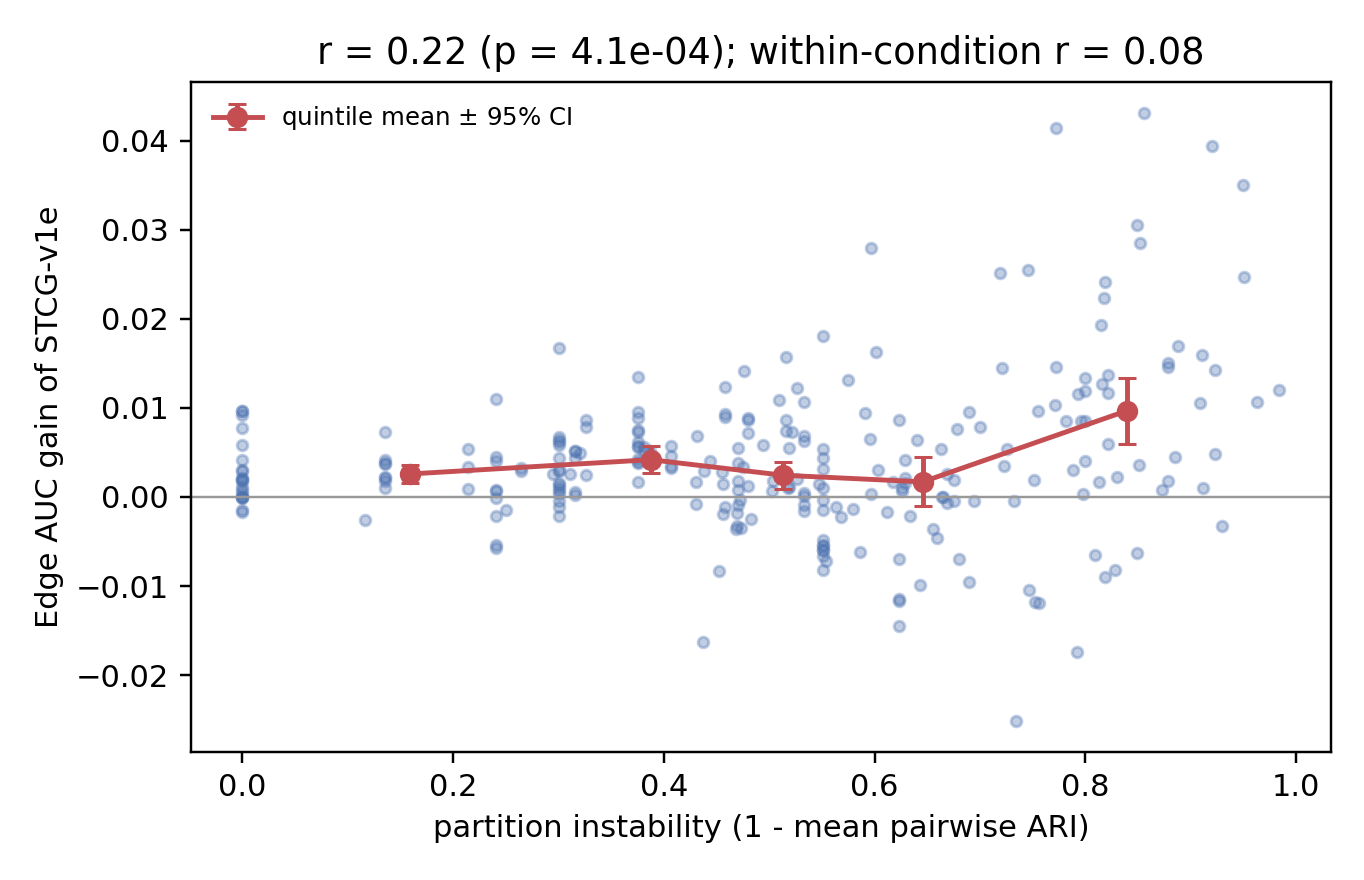
\includegraphics[width=\linewidth]{results/figures/stcg_ensemble_instability.png}
\caption{STCG-v1e gain against K-means partition instability across the 260 frozen stress fits. Points are individual fits; red markers are quintile means with 95\% confidence intervals. Instability predicts the gain across conditions ($r=0.22$, $p=4.1\times10^{-4}$) but not within them ($r=0.08$, $p=0.21$); baseline accuracy is weakly related ($r=0.11$, $p=0.078$). Restarts use seeds disjoint from the ensemble members.}
\Description{Scatter plot of ensemble gain versus partition instability with binned means and confidence intervals.}
\label{fig:ensemble-instability}
\end{figure}

\begin{table}[t]
\caption{Variance-reduced STCG-v1e against STCG-v1. $\Delta$ is the paired Edge AUC improvement; $p_t$ is the two-sided paired $t$-test; wins count seeds/cells where STCG-v1e is higher. The stress rows are subsets of the 13$\times$20 grid; the full table is in the artifact. Cell-level tests treat the 260 fits as independent; a seed-clustered test gives $p=2.1\times10^{-7}$ for the full grid.}
\label{tab:ensemble}
\centering
\small
\resizebox{\linewidth}{!}{\begin{tabular}{lrrrrr}
\toprule
Panel & STCG-v1 & STCG-v1e & $\Delta$ & $p_t$ & Wins \\
\midrule
Stationary VAR & 0.876 & 0.884 & $+0.0076$ & 0.0006 & 17/20 \\
Nonlinear VAR & 0.970 & 0.971 & $+0.0007$ & 0.191 & 14/20 \\
Switching VAR & 0.812 & 0.815 & $+0.0027$ & 0.032 & 13/20 \\
Stress grid (13$\times$20) & 0.797 & 0.801 & $+0.0041$ & $1.5\times10^{-12}$ & 190/260 \\
\quad switch period 300 & 0.815 & 0.831 & $+0.0161$ & $3.2\times10^{-5}$ & 17/20 \\
\quad $T{=}600$ & 0.763 & 0.768 & $+0.0044$ & 0.0008 & 16/20 \\
\quad $T{=}300$ & 0.657 & 0.661 & $+0.0034$ & 0.0027 & 14/20 \\
\bottomrule
\end{tabular}
}
\Description{Paired table comparing STCG-v1 and the twenty-partition score ensemble STCG-v1e on stationary, nonlinear, and switching generators, the full stress grid, and three stress subsets.}
\end{table}

\subsection{Specialist Stress Extension and Matched Timing}
\label{sec:exp-specialist-stress}

The main panel above fixes one switching configuration and twenty seeds; a frozen extension protocol preregisters the broader robustness check before any new result is observed.
It uses fresh generator seeds 100--119, disjoint from the main panel and the cMLP pilot seeds; retains the fixed algorithmic budgets; and supplies $K{=}2$ to both STCG-v1 and Regime-PCMCI.
Thirteen unique settings vary observation noise, sequence length, edge density, and switch period, following the original robustness and switch-difficulty axes (the switch-period cells use the periodic alternating switch at $T{=}1200$); five methods (STCG-v1, DynVAR-Lasso, VAR-Lasso, Regime-PCMCI, cMLP) are fitted on identical inputs.
All $1400$ planned fits across the stress and timing phases complete with zero failures or timeouts, so no conclusion rests on a missing specialist fit.
The primary family is the thirteen two-sided Regime-PCMCI Edge AUC contrasts under Holm correction; a second 52-test family covers all opponents, and the artifact retains every metric, paired seed set, and failure record.

\begin{table}[t]
\caption{Frozen specialist stress extension on fresh seeds 100--119: Edge AUC means (twenty paired seeds per cell) and the STCG-v1 minus Regime-PCMCI difference with 95\% CI. Fifteen displayed cells correspond to thirteen unique input settings; the base row repeats across axes. All $1400$ fits succeeded. After Holm correction over the thirteen primary contrasts, Regime-PCMCI wins at switch periods $150$/$300$ and $T{=}1500$; no cell favors STCG-v1 significantly.}
\label{tab:specialist-stress}
\centering
\small
\resizebox{\linewidth}{!}{\begin{tabular}{lrrrrrrl}
\toprule
Setting & $n$ & STCG & RPCMCI & cMLP & DynVAR & VAR & $\Delta$ vs RPCMCI [95\% CI] \\
\midrule
Noise 0 & 20 & 0.827 & 0.839 & 0.783 & 0.813 & 0.784 & $-0.012$ $[-0.025,+0.002]$ \\
Noise 0.05 & 20 & 0.827 & 0.838 & 0.783 & 0.813 & 0.784 & $-0.011$ $[-0.022,+0.001]$ \\
Noise 0.1 & 20 & 0.827 & 0.843 & 0.783 & 0.811 & 0.784 & $-0.016$ $[-0.027,-0.005]$ \\
Noise 0.2 & 20 & 0.821 & 0.830 & 0.778 & 0.804 & 0.779 & $-0.010$ $[-0.020,+0.002]$ \\
$T$ 300 & 20 & 0.657 & 0.618 & 0.544 & 0.658 & 0.640 & $+0.040$ $[+0.013,+0.067]$ \\
$T$ 600 & 20 & 0.763 & 0.759 & 0.667 & 0.769 & 0.729 & $+0.004$ $[-0.008,+0.016]$ \\
$T$ 1000 & 20 & 0.827 & 0.839 & 0.783 & 0.813 & 0.784 & $-0.012$ $[-0.025,+0.002]$ \\
$T$ 1500 & 20 & 0.852 & 0.876 & 0.824 & 0.837 & 0.824 & $-0.024$ $[-0.034,-0.013]$ \\
Density 0.1 & 20 & 0.828 & 0.816 & 0.788 & 0.814 & 0.788 & $+0.013$ $[-0.013,+0.040]$ \\
Density 0.18 & 20 & 0.827 & 0.839 & 0.783 & 0.813 & 0.784 & $-0.012$ $[-0.025,+0.002]$ \\
Density 0.3 & 20 & 0.802 & 0.816 & 0.750 & 0.790 & 0.751 & $-0.015$ $[-0.024,-0.005]$ \\
Density 0.45 & 20 & 0.765 & 0.773 & 0.709 & 0.761 & 0.709 & $-0.008$ $[-0.019,+0.004]$ \\
Period 150 & 20 & 0.741 & 0.849 & 0.787 & 0.732 & 0.789 & $-0.108$ $[-0.123,-0.091]$ \\
Period 300 & 20 & 0.815 & 0.853 & 0.785 & 0.817 & 0.786 & $-0.037$ $[-0.050,-0.023]$ \\
Period 600 & 20 & 0.834 & 0.848 & 0.785 & 0.820 & 0.786 & $-0.014$ $[-0.029,+0.005]$ \\
\bottomrule
\end{tabular}
}
\Description{Stress-extension table with one row per setting, showing Edge AUC for STCG-v1, Regime-PCMCI, cMLP, DynVAR-Lasso, and VAR-Lasso, plus the paired STCG-minus-specialist difference with its confidence interval.}
\end{table}

Table~\ref{tab:specialist-stress} replicates the operating point and bounds it.
On the base single-switch configuration with new seeds, STCG-v1 and Regime-PCMCI remain statistically tied (Edge AUC $0.827$ versus $0.839$; difference $-0.0121$, 95\% CI $[-0.0248, 0.0022]$, Holm $p_t=0.571$).
The tie does not survive the stress axes.
Regime-PCMCI is decisively stronger under fast switching: the gap reaches $-0.1078$ Edge AUC at switch period $150$ (Holm $p_t=1.1\times10^{-9}$) and $-0.0375$ at period $300$ ($p_t=4.6\times10^{-4}$), consistent with the mixed-window failure mode of Section~\ref{sec:analysis}.
It is also stronger on the longest sequences ($T{=}1500$: $-0.0240$, Holm $p_t=0.0027$), where its joint fit pools more samples per regime, and borderline-ahead at density $0.30$ ($-0.0147$, Holm $p_t=0.066$).
STCG-v1's only nominally positive cell is $T{=}300$ ($+0.0398$, 95\% CI $[0.0131, 0.0666]$), which does not survive Holm correction ($p_t=0.082$); all noise levels, the remaining densities, $T{=}600$, and period $600$ are ties.
Parity with the specialist is therefore an operating-point result: with a supplied regime count, the annealed specialist is stronger under fast switching and long sequences, and we report this boundary rather than an average win rate.

\begin{table}[t]
\caption{Dedicated matched timing on the base switching configuration (fresh seeds 100--119, one worker, exclusive machine, fit boundary only). Ratios are geometric means of opponent over STCG-v1 per-seed fit times with 95\% CIs. The base condition is noise-free, whereas Table~\ref{tab:all-methods}'s fit times come from the noise-0.10 descriptive panel; the two protocols should not be mixed. Ratios collected inside the concurrent stress grid are descriptive-only and excluded.}
\label{tab:specialist-timing}
\centering
\small
\resizebox{\linewidth}{!}{\begin{tabular}{lrlrl}
\toprule
Method & Fits & Seconds: median [IQR] & Ratio $n$ & Geometric cost / STCG [95\% CI] \\
\midrule
STCG-v1 & 20/20 & 0.0317 [0.0299, 0.0334] & -- & Reference \\
Regime-PCMCI & 20/20 & 166.8963 [162.8269, 171.8444] & 20 & 5575.36 [5245.67, 5983.95] \\
cMLP & 20/20 & 2.6500 [2.6143, 2.7042] & 20 & 86.55 [81.83, 92.06] \\
DynVAR-Lasso & 20/20 & 0.0145 [0.0137, 0.0152] & 20 & 0.46 [0.43, 0.49] \\
VAR-Lasso & 20/20 & 0.0035 [0.0034, 0.0037] & 20 & 0.12 [0.11, 0.12] \\
\bottomrule
\end{tabular}
}
\Description{Matched timing table listing each method's completed fits, median and quartile fit seconds, and the geometric-mean cost ratio against STCG-v1 with its confidence interval.}
\end{table}

A dedicated timing phase repeats the base configuration on identical inputs with one worker and an exclusive machine, timing only each method's fit boundary (standardization, lag design, target fits, state inference, aggregation).
Table~\ref{tab:specialist-timing} shows the cost profile behind the tie: Regime-PCMCI's wall-clock cost is $5575\times$ STCG-v1's (95\% CI $[5246, 5984]$; CPU-time ratio $6293\times$), cMLP costs $86.6\times$ ($[81.8, 92.1]$), and the Lasso baselines are faster than STCG-v1 itself (geometric ratios $0.458$ for DynVAR-Lasso and $0.116$ for VAR-Lasso).
STCG-v1 is therefore mid-pack in absolute cost; its advantage over the specialist is a wall-clock difference of more than three orders of magnitude at the operating point where recovery is tied, not universal cheapness. Because the descriptive panel and this matched phase use different noise levels and machine load, ratios should be read from Table~\ref{tab:specialist-timing}, not recomputed from Table~\ref{tab:all-methods}.

\subsection{Real-Data Regime Recovery and Diagnostic Probes}
\label{sec:exp-real}

Real benchmarks use nine datasets: four ETT files~\cite{zhou2021informer}, BeijingPM25 from the Beijing multi-site air-quality data~\cite{zhang2017cautionary}, OccupancySensors from UCI Occupancy Detection~\cite{candanedo2016occupancydata,candanedo2016accurate}, AReMActivities from UCI AReM~\cite{palumbo2016arem}, UCIHARWindowSignals from UCI smartphone activity recognition~\cite{reyesortiz2012har}, and HydraulicSystems from UCI hydraulic condition monitoring~\cite{helwig2018hydraulic}.
They cover 17,420--69,680 ETT samples, 35,064 hourly PM2.5 observations, 20,560 minute-level room-sensor observations, 42,237 ordered AReM wearable-sensor samples, 10,299 UCI HAR inertial-signal windows, and 132,300 one-second Hydraulic Systems sensor rows from 2,205 test cycles.
Forecasting, forward state prediction, and warning evaluation use chronological protocols. Full-series alignment and capped-segment recovery are descriptive: external labels determine segment placement and the supplied count in the latter, while assignments within each segment are estimated from sensor data. Historical random-window label prediction is reported separately as an optimistic retrospective diagnostic.
We order the evidence to match the paper's claim: regime recovery on labeled systems first, state--label alignment second, explicit boundaries third, and forecasting last as a clearly labeled diagnostic.

\subsubsection{Head-to-Head Regime Discovery on Labeled Transition Segments}
\label{sec:exp-real-headtohead}

The most direct real-data test of the paper's claim uses the two datasets with ground-truth operating-mode labels, HydraulicSystems and AReMActivities.
Each configuration caps a $1500$-sample window centered on the first ground-truth transition (or block-concatenates four single-activity recordings for the concat-4 configuration). All methods see the identical capped window and receive the same annotated regime-count setting. STCG-v1 uses that count with an acceptance threshold of zero, so this experiment evaluates assignments at supplied $K$, not selection of an unknown count. Control configurations instead supply the number of regimes actually present in the capped segment to every method.
Regime-PCMCI uses the synthetic runner's fixed budget; metrics are window-level ARI and Hungarian-aligned accuracy over window-majority labels, with STCG-v1 recomputed over five seeds and the compute-bound specialists over two.

\begin{table}[t]
\caption{Descriptive regime recovery on capped real transition segments: window-level ARI with aligned accuracy in parentheses. All methods receive the indicated $K$; ``present'' is the number of regimes in the segment. STCG's acceptance threshold is zero. MSAR-X is the legacy independent-equation control, not joint MSVAR. $^{\dagger}$MSAR-X exceeded the per-call compute budget (two attempts, 295 s each). $^{\ddagger}$No Regime-PCMCI annealing converged on either seed. --- marks unrun combinations.}
\label{tab:real-regime}
\centering
\small
\resizebox{\linewidth}{!}{\begin{tabular}{lccc}
\toprule
Segment ($K$ given; present) & STCG-v1 & Regime-PCMCI & MSAR-X \\
\midrule
Hydraulic cooler (3; 2) & \textbf{0.769} (0.778) & 0.000 (0.556) & budget$^{\dagger}$ \\
Hydraulic cooler, $K{=}2$ present (2; 2) & \textbf{0.822} (0.956) & 0.000 (0.556) & --- \\
Hydraulic valve (4; 3) & \textbf{0.171} (0.778) & no conv.$^{\ddagger}$ & --- \\
Hydraulic valve, $K{=}3$ present (3; 3) & \textbf{0.282} (0.844) & no conv.$^{\ddagger}$ & --- \\
AReM bending (2; 2) & \textbf{0.241} (0.778) & 0.000 (0.556) & 0.000 (0.556) \\
AReM concat-4 (4; 4) & 0.094 (0.556) & \textbf{0.571} (0.778) & --- \\
\bottomrule
\end{tabular}
}
\Description{Head-to-head regime recovery table comparing STCG-v1, Regime-PCMCI, and the legacy MSAR-X control on four contiguous hydraulic and activity transition segments plus one concatenated activity configuration.}
\end{table}

Table~\ref{tab:real-regime} shows that STCG-v1 wins every completed contiguous-segment fit.
On the Hydraulic cooler transition, Regime-PCMCI collapses to a single regime (ARI $0.000$) even on the easier $K{=}2$-present control segment, where STCG-v1 reaches ARI $0.822$ with aligned accuracy $0.956$.
On the valve transition, Regime-PCMCI's annealed search finds no feasible solution at either regime count on either seed.
The legacy MSAR-X control collapses on the one configuration whose fit completes (AReM bending, about $260$ s per fit) and exceeds the compute budget on cooler; neither result establishes superiority over joint MSVAR.
Per-fit compute on the capped segments is $46$--$98$ s for Regime-PCMCI versus $0.01$--$0.08$ s for STCG-v1 state inference, roughly three orders of magnitude.
The one loss is the constructed AReM concat-4 configuration, where Regime-PCMCI reaches ARI $0.571$ against STCG-v1's $0.094$; we return to it as a boundary condition below, noting that only 2 of its 10 annealings per seed were error-free, so the figure carries optimizer noise.

\subsubsection{State--Label Alignment on Full Real Series}
\label{sec:exp-real-alignment}

Over the full 132,300-sample Hydraulic series, STCG-v1's supplied $K{=}2$ partition passes the automatic gate and aligns with the three-level cooler operating condition at ARI $0.735 \pm 0.006$ and aligned accuracy $0.902 \pm 0.002$ over five seeds, with no label access during assignment.
The separate label-free state-count selector of Section~\ref{sec:method-variants} chooses $K{=}3$ on all five seeds. In the historical random-window diagnostic, state mapping reaches balanced accuracy $0.948 \pm 0.004$, graph-score centroid features $0.959 \pm 0.003$, and the supervised sensor-feature ceiling $0.994 \pm 0.004$. These figures are optimistic because state fitting uses the full series and windows overlap; they are not forward predictive evidence.
A forward-only variant fits graph-state centroids and state--label mappings on chronological train windows only and assigns future windows to the train-fitted centroids: late-future cooler windows are predicted at balanced accuracy $0.953 \pm 0.003$ (centroids $0.966$, ceiling $1.000$).
This forward result is encouraging but narrow---the future cooler segment contains only the late-life condition---and the multi-class valve forward check stays at the train-majority level ($0.250$ balanced accuracy, centroid features $0.323$).
On AReM, the default $K{=}2$ states partially align with activity blocks (ARI $0.251$, aligned accuracy $0.487$ against six present labels); a threshold sweep reaches ARI $0.309 \pm 0.035$ at $K{=}3$, and at $K{=}4$ the windowed graph-score features carry substantial activity information (supervised centroid balanced accuracy $0.623 \pm 0.033$ versus a $0.143$ majority baseline), while the compact unsupervised state mapping is weaker ($0.421$) and the sensor-feature ceiling reaches $0.810$.
The label-free selector picks coarse $K{=}2$ AReM states on all five seeds ($0.283 \pm 0.005$ balanced accuracy against seven activity labels), so AReM's fine-grained activities are not naturally recovered by the compact state objective.

\subsubsection{Boundaries: Concatenation, Collapse, and Label--Window Mismatch}
\label{sec:exp-real-boundaries}

Three tracked failures bound the real-data claim.
First, the AReM concat-4 loss above: when regime boundaries coincide with large level shifts between concatenated recordings, the specialist's annealed assignment exploits them and our score clustering does not.
Second, on OccupancySensors the auto gate rejects every multi-state partition on all seeds (single inferred state, ARI $0.000$, aligned accuracy $0.737$ equal to the majority window-label rate): binary occupancy is simply not expressed in lagged graph structure at this granularity.
Third, on UCIHARWindowSignals inference collapses to one state with mean window label purity $0.230$: the sliding windows already mix activities, so the label stream is mismatched to the windowing before clustering begins, and the best non-collapsed low-threshold setting reaches only ARI $0.090$.

\subsubsection{Forward Diagnosis at Prespecified Time Origins}
\label{sec:real-fixed-origins}

To remove label-sighted interval selection, a separate protocol fixes training endpoints at 20\%, 40\%, 60\%, and 80\% of each series and tests the next 20\%.
Complete 300-sample windows do not cross split boundaries or overlap other test windows; diagnosis observes each window before predicting its label.
Feature scaling across windows, centroids, classifiers, and state--label maps use training windows only.
STCG uses either the same supplied $K{=}2$ on both datasets or an explicitly separate training-silhouette selector over $K=2,\ldots,6$, followed by the unchanged gate.
All origins are retained, including unseen test classes. Five initialization seeds are averaged within each origin; the four origins share training history, so we report descriptive means rather than treating them as independent replicates.

\begin{table}[t]
\caption{Forward balanced accuracy, averaged over four prespecified time origins. Cooler has two multi-class test blocks; valve and AReM have four. AReM follows archival recording order, with unseen activities and recording-crossing windows, rather than a natural online stream.}
\label{tab:real-fixed-origins}
\centering
\small
\begin{tabular}{lrrr}
\toprule
Method & Cooler & Valve & AReM \\
\midrule
Train majority & 0.125 & 0.250 & 0.000 \\
Sensor centroid & 0.750 & 0.268 & 0.438 \\
Graph centroid & 0.724 & 0.320 & 0.282 \\
Sensor logistic & 0.750 & 0.265 & 0.422 \\
STCG, fixed $K{=}2$ & 0.250 & 0.250 & 0.110 \\
STCG, train-selected $K$ & 0.298 & 0.250 & 0.110 \\
\bottomrule
\end{tabular}

\Description{Fixed-origin forward diagnosis comparing six methods on Hydraulic cooler, Hydraulic valve, and AReM. Simpler sensor or graph-feature classifiers outperform the compact STCG state mappings.}
\end{table}

Table~\ref{tab:real-fixed-origins} does not establish practical superiority of graph-state mapping.
On valve, all four test blocks contain four classes already observed in training: STCG reaches balanced accuracy $0.250$, equal to training-majority prediction, versus graph centroids $0.320$.
On cooler, fixed-$K$ STCG reaches $0.250$ and the training-selected variant $0.298$, versus sensor centroids $0.750$; new conditions appear in the two multi-class blocks.
AReM STCG reaches $0.110$ versus sensor centroids $0.438$, with a mean unseen-class fraction $0.634$ and 70 of 112 test windows crossing recording boundaries.
These results limit the earlier selected-segment alignment claim: association with operating labels does not ensure a useful compact forward diagnostic.

A companion check fixes four disjoint 1500-sample intervals per dataset at 10\%, 35\%, 60\%, and 85\% of series length, independently of labels, with five nonoverlapping windows per interval.
All three methods receive $K{=}2$ and retain their default fit settings; STCG retains its default gate.
STCG and sensor KMeans complete all eight intervals, whereas every Regime-PCMCI fit reaches the predeclared 120-second worker limit, including process startup. These resource-limited outcomes supply no fitted-specialist superiority comparison, and the timing boundaries are not suitable for a speed ratio.
All cooler and AReM intervals have one true state but both completed methods infer two, giving ARI zero. On the three multi-state valve window tasks, mean ARI is $-0.142$ for STCG versus $0.074$ for sensor KMeans.
The full segment and failure records are retained in the artifact; these fixed intervals do not reproduce the positive alignment evidence from the earlier label-centered intervals.

\subsubsection{Forecasting and Transition Warning as Diagnostic Probes}
\label{sec:exp-real-forecasting}

Table~\ref{tab:real-forecasting} reports one-step forecasting RMSE under chronological splits with graph scores fit on the training segment only.
Dense ridge or persistence is strongest on every dataset among materially distinct models; on OccupancySensors, persistence wins by $1.76\times 10^{-4}$ RMSE, below the $0.001$ threshold used for meaningful real-data gains.
STCG-v1 hard graph masks approximately tie the DynVAR-Lasso mask (HydraulicSystems RMSE $0.470$ versus $0.472$) and never beat dense ridge or persistence, and a hard-mask sweep over graph fraction, Lasso strength, and window size finds no exception; the non-self dense baseline also underperforms, indicating that self-lag features carry these forecasting splits.
Soft graph-weighted ridge avoids the deletion effect: the weight sweep finds a meaningful AReMActivities gain of $0.0034$ RMSE over tuned dense ridge (all other datasets below threshold), and under tuned $K{=}4$ states STCG-v1 improves weighted RMSE from DynVAR-Lasso's $0.9062$ to $0.9041$---four of five seeds improve, but the paired test is not statistically confirmed (paired $t$ $p=0.142$, one-sided Wilcoxon $p=0.0625$).
The learned top edges remain interpretable load/temperature-channel, station-to-station, room-sensor, activity-sensor, and hydraulic-sensor relations.
The ETTh1 STCG-v1 mask cell ($0.760$) reflects a KMeans numeric flip in the recreated environment, where ETTh1 auto-state inference now selects two states; no claim rests on it.
We therefore treat real forecasting strictly as a leakage-controlled diagnostic, not as evidence of predictive gains.

The chronological Hydraulic transition-warning pilot---features from past cycles only, with horizon-sized purges before validation and test boundaries---is likewise mixed.
Sensor-plus-graph logistic regression reaches AP $0.901$ and ROC AUC $0.752$ on 10-cycle valve-condition warnings versus majority AP $0.742$. On 10-cycle stable-flag warnings, sensor-plus-graph AP is $0.278$, graph-only ridge AP $0.275$, and majority AP $0.244$.
Selected STCG-v1 state features are best by AP only at short horizons (5-cycle stable-flag $0.160$ versus $0.128$; 3-cycle valve-condition $0.239$ versus $0.222$) and best by F1 on 10-cycle valve-condition warnings ($0.864$). The validation-selected ablation now chooses the default lookback/window configuration for sensor-plus-STCG on 10-cycle stable-flag warnings: AP $0.272$ versus sensor-only $0.278$ at the same lookback. Selected sensor-plus-STCG reaches $0.834$ on 10-cycle valve warnings, below the default sensor-plus-graph $0.901$. These ablations use the corrected positive-score selection rule; both the earlier boundary purge and the subsequent zero-score fallback repair are recorded separately in the artifact.
This is bounded pilot evidence that graph states carry warning-relevant signal at some horizons, not a deployment result.

\begin{table}[t]
\caption{Real benchmark one-step forecasting RMSE on ETT small, BeijingPM25, OccupancySensors, AReMActivities, UCIHARWindowSignals, and HydraulicSystems datasets, reported as a leakage-controlled diagnostic. Mask columns use hard graph feature selection; weight columns use graph-weighted ridge. Lower is better.}
\label{tab:real-forecasting}
\centering
\small
\resizebox{\linewidth}{!}{\begin{tabular}{lrrrrrr}
\toprule
Dataset & Persistence & Dense & DynVAR Mask & DynVAR Weight & STCG Mask & STCG Weight \\
\midrule
AReMActivities & 1.128 & 0.912 & 1.259 & 0.912 & 1.230 & 0.912 \\
BeijingPM25 & 0.266 & 0.233 & 0.367 & 0.233 & 0.367 & 0.233 \\
ETTh1 & 0.439 & 0.409 & 0.728 & 0.409 & 0.760 & 0.409 \\
ETTh2 & 0.246 & 0.227 & 0.888 & 0.227 & 0.888 & 0.227 \\
ETTm1 & 0.253 & 0.242 & 0.695 & 0.242 & 0.695 & 0.242 \\
ETTm2 & 0.156 & 0.149 & 0.802 & 0.149 & 0.802 & 0.149 \\
HydraulicSystems & 0.167 & 0.155 & 0.472 & 0.156 & 0.470 & 0.156 \\
OccupancySensors & 0.046 & 0.046 & 0.744 & 0.046 & 0.744 & 0.046 \\
UCIHARWindowSignals & 0.852 & 0.680 & 0.811 & 0.680 & 0.811 & 0.680 \\
\bottomrule
\end{tabular}
}
\Description{Real benchmark forecasting table reporting RMSE for persistence, dense ridge, DynVAR graph masks and weights, and STCG graph masks and weights across nine datasets.}
\end{table}

Table~\ref{tab:evidence-summary} summarizes how the main results should be read.
\begin{table}[t]
\caption{Evidence summary across synthetic and real probes.}
\label{tab:evidence-summary}
\centering
\small
\resizebox{\linewidth}{!}{\begin{tabular}{lll}
\toprule
Probe & Evidence & Reading \\
\midrule
Switching synthetic & Close STCG/Regime-PCMCI estimates; no equivalence claim & Supplied-count recovery \\
Stationary/nonlinear & Global VAR/Granger/PCMCI/cMLP stronger & Boundary condition \\
Real regime recovery & Annotated $K$ given to every method; concat-4 favors specialist & Descriptive alignment \\
Real forecasting & Dense ridge or persistence strongest; AReM gain unconfirmed & Diagnostic only \\
Fixed-origin diagnosis & Compact states trail sensor or graph centroids & No established utility advantage \\
Fixed real intervals & Weak alignment; all specialist fits hit fixed budget & Negative boundary evidence \\
Transition warning & Purged boundaries and safe null selection; selected horizons help & Bounded pilot \\
Gate stress & Fallback matters; stationary and rare-state failures remain & Empirical heuristic \\
\bottomrule
\end{tabular}
}
\Description{Summary table grouping the evidence into switching synthetic recovery, non-switching recovery, real regime recovery, real forecasting, graph-state diagnosis, and transition warning, with the interpretation for each probe.}
\end{table}

\subsection{Ablation: State Aggregation Is the Mechanism}
\label{sec:exp-ablation}

Focused ablations test whether the switching-regime gain comes from ordinary windowing, latent graph-state aggregation, or the optional state-contrast term.

\begin{table}[t]
\caption{Focused ablation on twenty-seed switching-regime recovery. The gain comes from latent graph-state clustering rather than windowing alone.}
\label{tab:state-ablation}
\centering
\small
\begin{tabular}{lrrr}
\toprule
Variant & Edge AUC & P@K & SHD \\
\midrule
DynVAR-Lasso & 0.798 & 0.646 & 38.6 \\
STCG-v1/no-state & 0.798 & 0.646 & 38.6 \\
STCG-v1/state-only & \textbf{0.812} & \textbf{0.673} & \textbf{35.5} \\
STCG-v1/state+contrast & 0.808 & 0.665 & 36.4 \\
\bottomrule
\end{tabular}
\Description{Ablation table comparing DynVAR-Lasso, STCG-v1 without state aggregation, STCG-v1 with state-only aggregation, and STCG-v1 with the optional state-contrast term.}
\end{table}

The ablation in Table~\ref{tab:state-ablation} isolates the mechanism.
Removing state clustering collapses the method exactly to the dynamic window baseline, while inferred state aggregation improves Edge AUC and SHD.
The contrast term is therefore treated as a negative ablation rather than a core contribution.
Section~\ref{sec:analysis} complements this mechanism ablation with a one-factor-at-a-time isolation of the remaining heuristic knobs.

\section{Analysis}
\label{sec:analysis}

\begin{figure}[t]
\centering
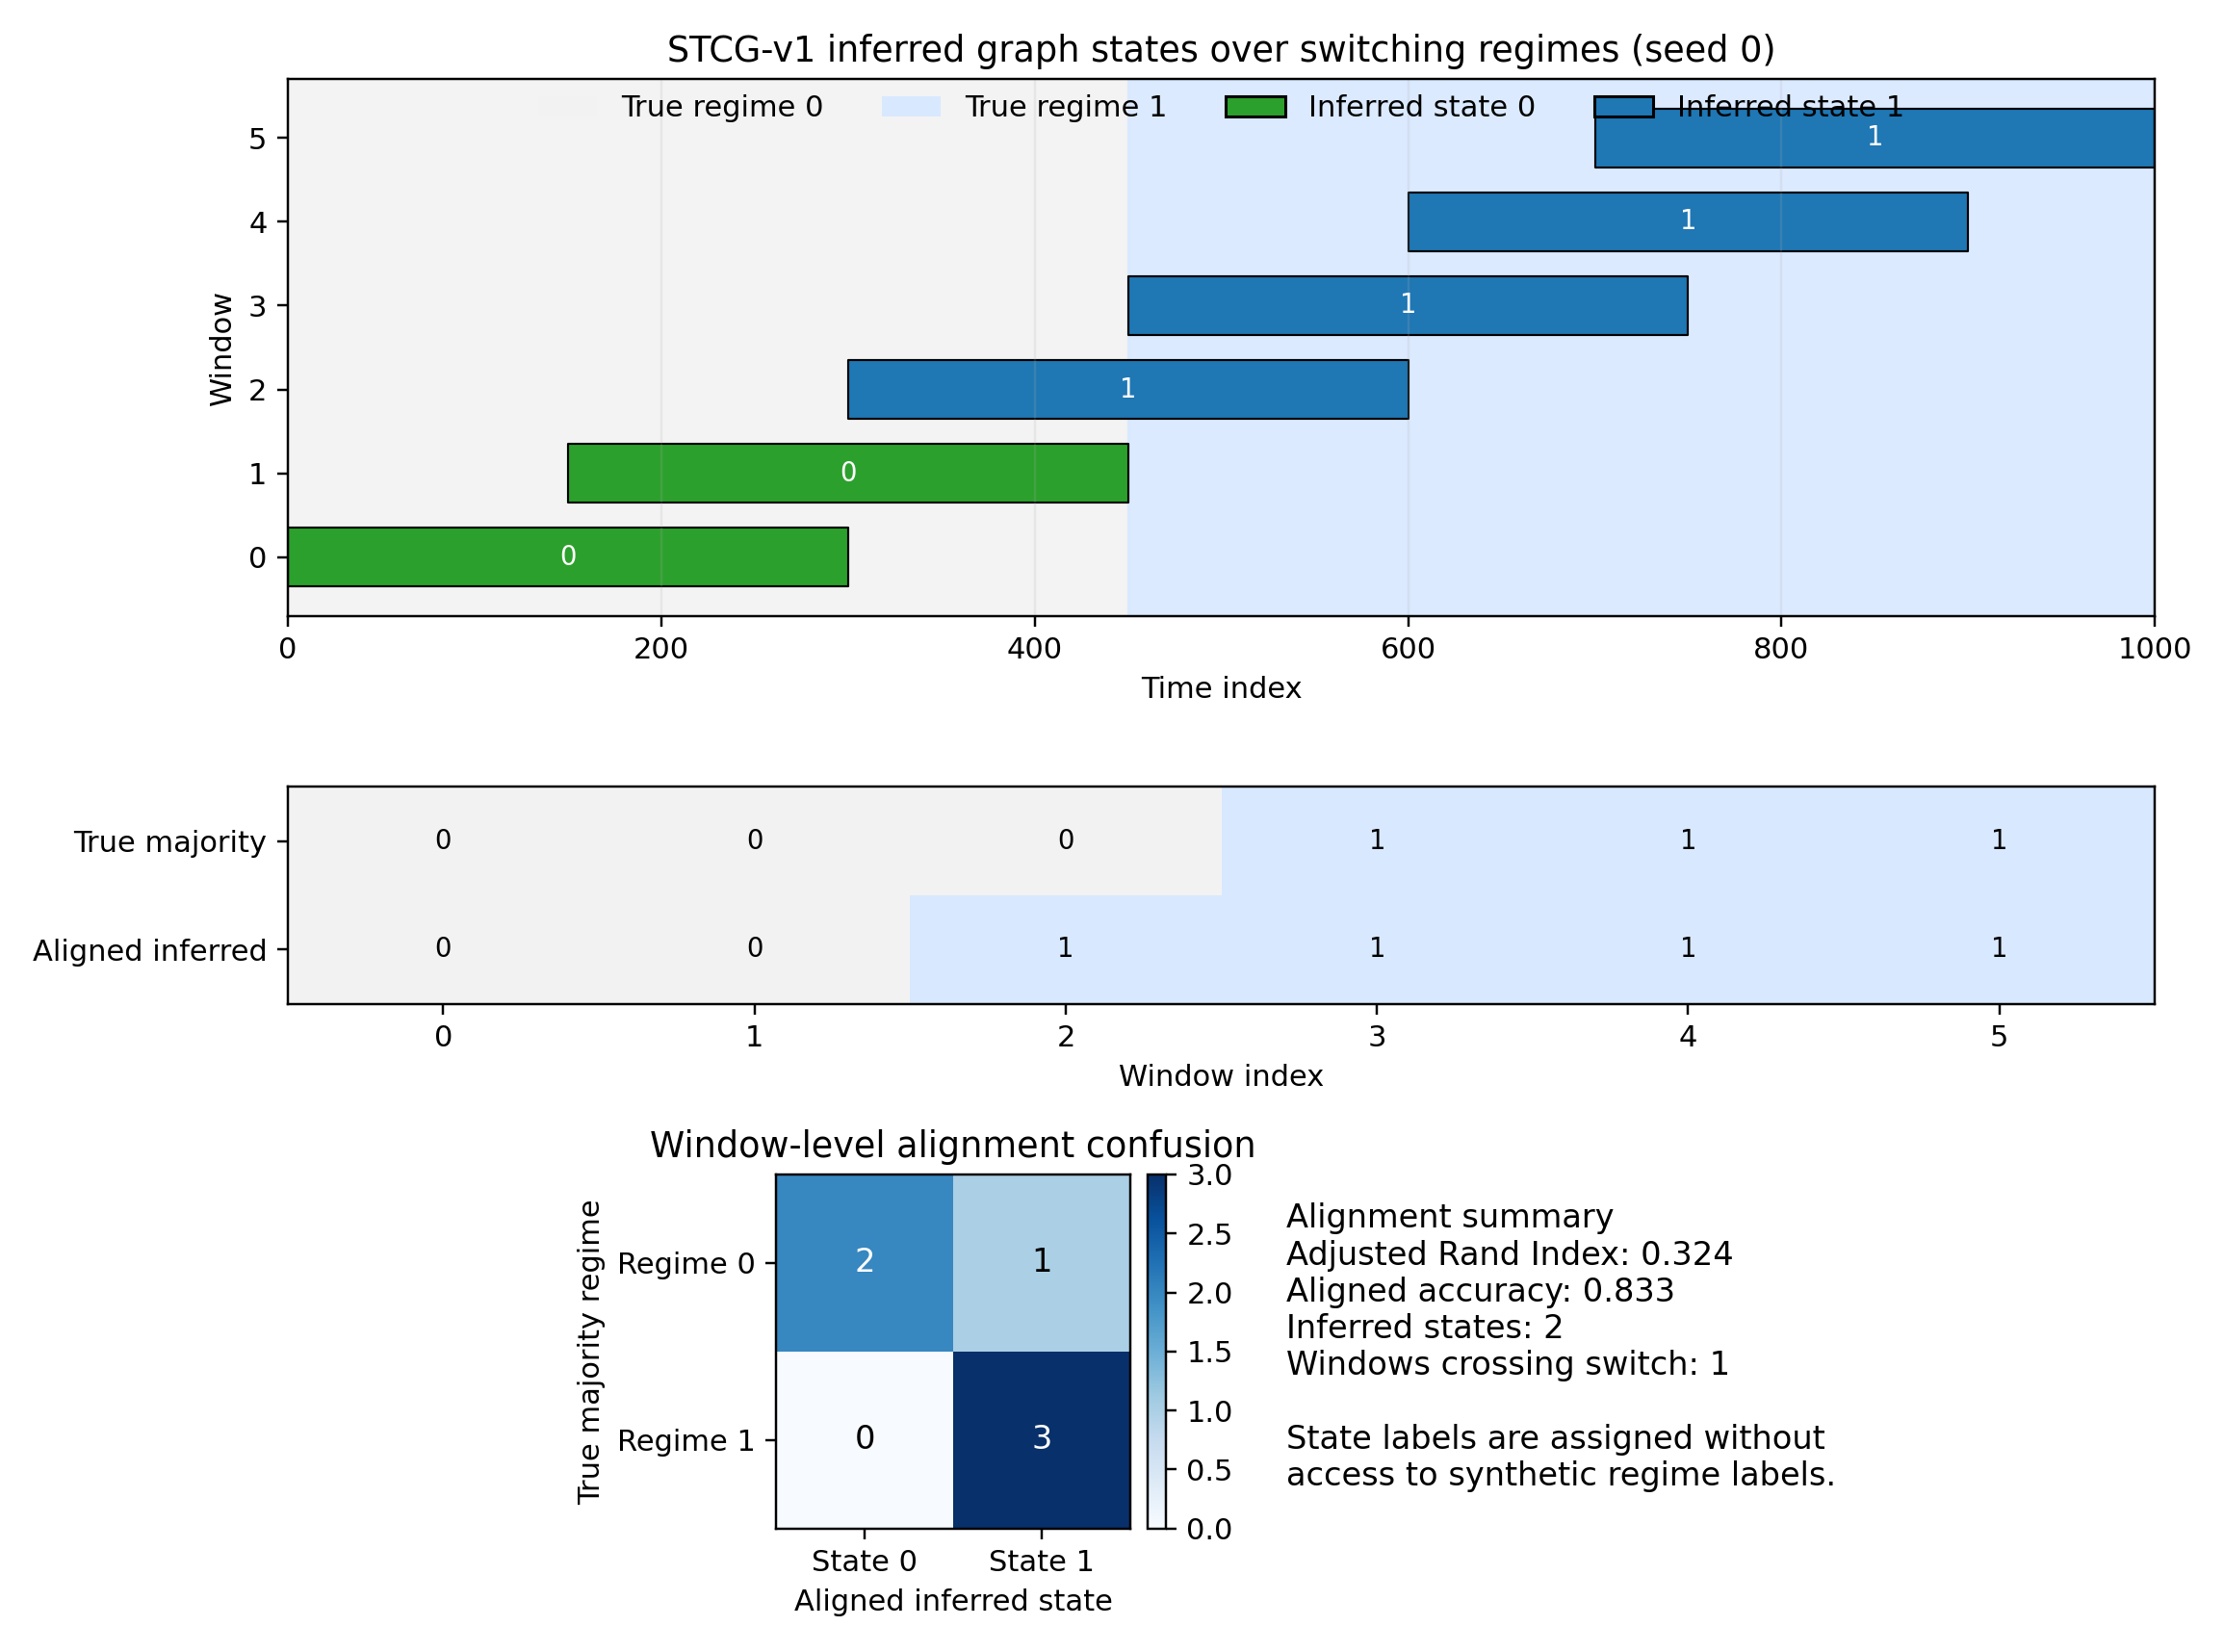
\includegraphics[width=\linewidth]{results/figures/stcg_v1_state_diagnostics_seed0.png}
\caption{Window-level graph-state diagnostics for a switching synthetic run. STCG-v1 infers states without regime labels; after label alignment, the only seed-0 mismatch is the window crossing the true switch boundary.}
\Description{Timeline and confusion-matrix diagnostic comparing inferred STCG graph states with hidden switching regimes.}
\label{fig:state-diagnostics}
\end{figure}

The state diagnostic in Figure~\ref{fig:state-diagnostics} checks whether the inferred clusters correspond to meaningful regime changes.
Across five seeds, STCG-v1 infers two states in every run, reaches aligned state accuracy $0.900 \pm 0.091$, and achieves Adjusted Rand Index $0.595 \pm 0.370$.
Lower ARI cases are mainly caused by windows that straddle the true switching boundary.

Robustness sweeps over observation noise, sequence length, and edge density compare STCG-v1 with VAR-Lasso and DynVAR-Lasso; the frozen specialist extension of Section~\ref{sec:exp-specialist-stress} repeats these axes on fresh seeds with Regime-PCMCI and cMLP included.
STCG-v1 obtains the best Edge AUC in 10 of 12 sweep settings over twenty seeds.
It is best at all tested observation-noise levels and at all four tested edge densities (including the sparsest, $0.10$), but short sequences of 300 and 600 timesteps still favor DynVAR-Lasso.
The main failure mode is therefore limited temporal evidence: if a window has too few samples or mixes regimes heavily, state inference becomes less reliable.
The switch-difficulty sweep makes this boundary explicit.
When the regime switch period is 150 timesteps with 300-step windows, oracle window purity falls to $0.500$ and STCG-v1 and DynVAR-Lasso have nearly identical Edge AUC ($0.733$). STCG still accepts two states here; this is not a gate fallback.
At a 600-step switch period, oracle purity rises to $0.929$, STCG-v1 reaches Edge AUC $0.847$, and the oracle upper bound is $0.849$ versus DynVAR-Lasso $0.835$.

\paragraph{Knob isolation.}
The mechanism ablation of Section~\ref{sec:exp-ablation} leaves open whether the remaining heuristic knobs of Table~\ref{tab:knob-map} (Section~\ref{sec:method-knobs}) are load-bearing.
Table~\ref{tab:knob-ablation} isolates them one factor at a time on the switching generator over twenty seeds (Figure~\ref{fig:knob-ablation}).
The auto-gate thresholds are never binding: the weakest per-seed clustering-improvement signal ($\approx 0.270$) still clears the largest tested inertia threshold ($0.18$), so all seven gate configurations accept the supplied $K{=}2$ on all twenty seeds and reproduce the default $0.812$ Edge AUC exactly.
Including actual self-lag coefficients in the clustering features gives Edge AUC $0.813$ versus the default $0.812$, with state ARI $0.730$ versus $0.764$ over these twenty seeds; final graph scores still exclude self-edges. Adding window statistics leaves the default recovery scores unchanged. Aggregator means range from $0.798$ to $0.814$; the best tested mean (cross-state p90, $0.814$) is slightly above the default ($0.812 \pm 0.047$), without an optimality claim.
Window size has a larger effect: on a period-300 switcher, $h{=}300$ maximizes Edge AUC ($0.781$ versus $0.748$ at $h{=}150$ and $0.765$ at $h{=}450$), yet state ARI collapses for $h \geq 300$ ($0.035$ and $0.050$, versus $0.333$ at $h{=}150$) because windows then straddle regime boundaries.
State aggregation therefore improves edge recovery even where the inferred states no longer track the true regimes---the gain does not hinge on exact regime recovery, consistent with the oracle diagnostic of Section~\ref{sec:exp-synthetic-results}.

\begin{table}[t]
\caption{One-factor-at-a-time isolation of the heuristic knobs of Table~\ref{tab:knob-map} on switching-regime recovery (twenty seeds). Edge AUC is the range of group means; the default configuration reconciles with Table~\ref{tab:all-methods}.}
\label{tab:knob-ablation}
\centering
\small
\resizebox{\linewidth}{!}{{\sloppy\setlength{\tabcolsep}{3pt}\begin{tabular}{p{0.17\linewidth}p{0.26\linewidth}rp{0.32\linewidth}}
\toprule
Knob group & What varies & Edge AUC & Finding \\
\midrule
Gate thresholds & inertia $0.06$--$0.18$, coherence $0.45$--$0.65$, share $0.05$--$0.15$ & 0.812--0.812 & Never binding: weakest per-seed improvement $\approx 0.270$ still clears $0.18$; $K{=}2$ on 20/20 seeds in all 7 configs \\
Aggregation & within-state mean / median / p75 / max; cross-state max / mean / p90 & 0.798--0.814 & Best tested mean (cross p90, $0.814$) slightly above default ($0.812$); no optimality claim \\
State features & non-self vs all scores; $+$ window stats & 0.812--0.813 & Actual self-lag features: ARI 0.730 vs default 0.764; window stats leave recovery unchanged \\
Window size $h$ & $150/300/450$, stride $h/2$, switch period 300 & 0.748--0.781 & $h{=}300$ best (0.781) but state ARI collapses at $h \geq 300$ (0.035/0.050 vs 0.333 at $h{=}150$): windows straddle switches \\
\bottomrule
\end{tabular}}
}
\Description{Knob ablation table with one row per knob group---auto-gate thresholds, aggregators, state features, and window size---showing the edge AUC range across configurations and the finding for each group.}
\end{table}

\begin{figure}[t]
\centering
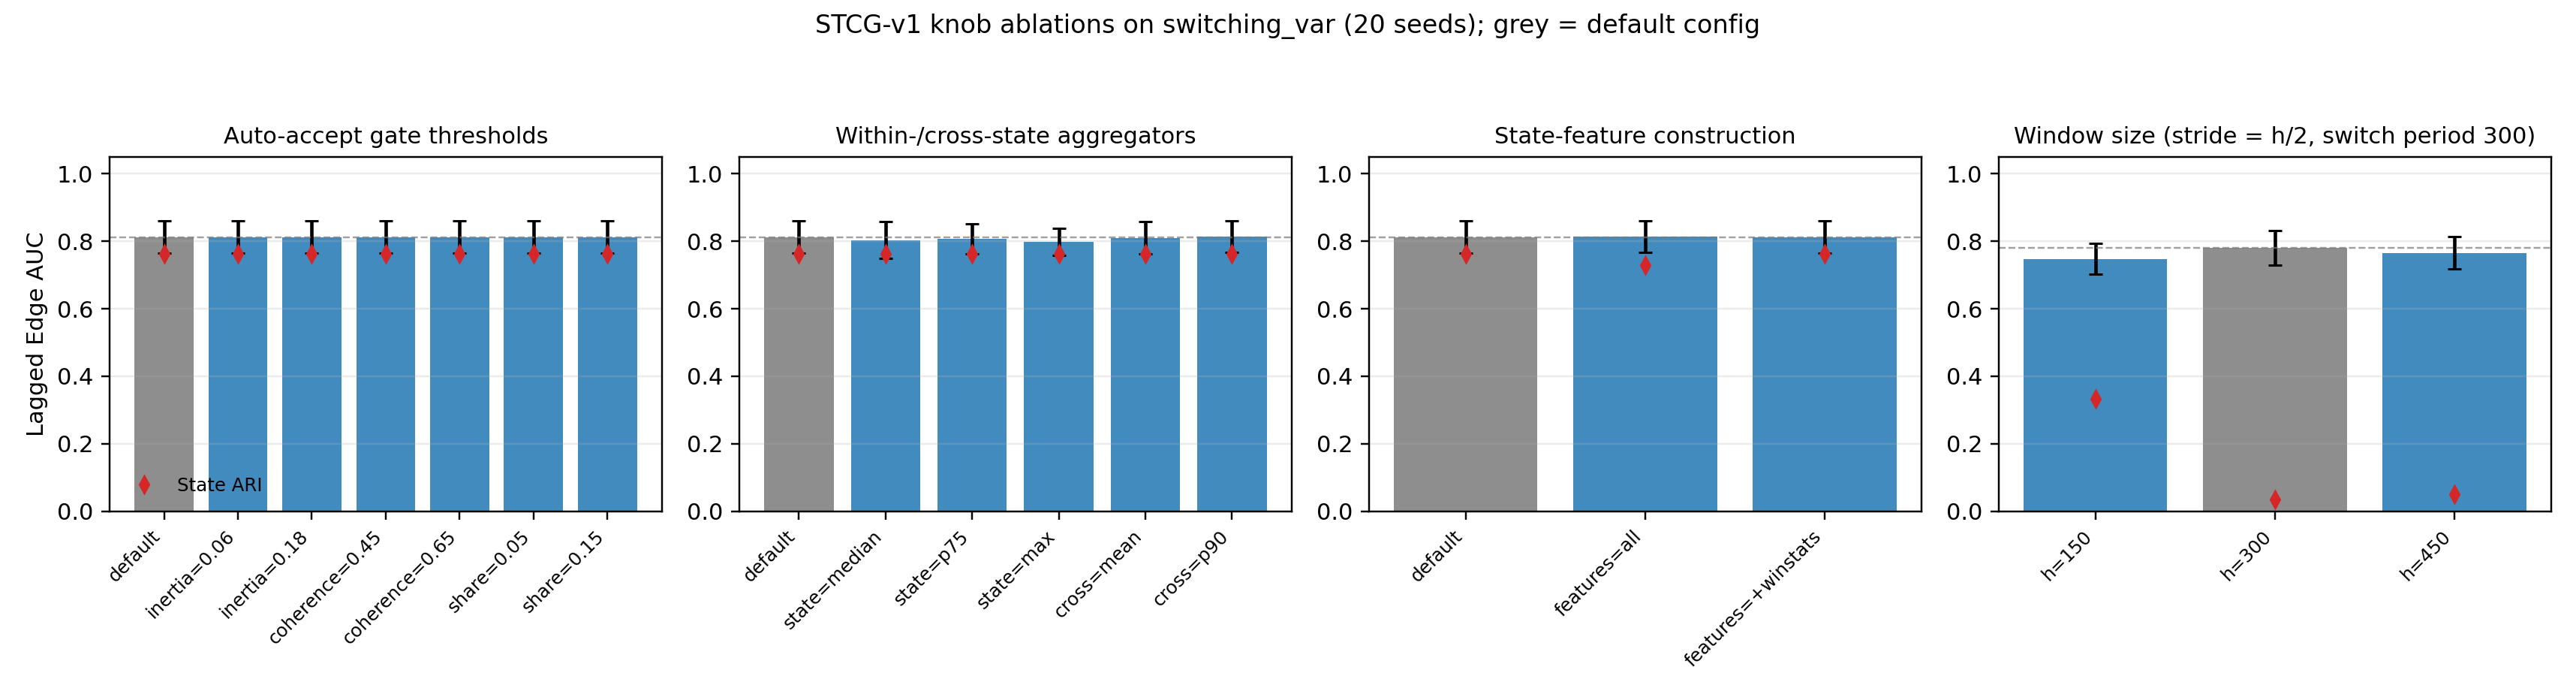
\includegraphics[width=\linewidth]{results/figures/stcg_knob_ablation_edge_auc.png}
\caption{Edge AUC across the knob-ablation configurations on the switching generator (twenty seeds). Gate variants reproduce the default, self-lag features change assignments with a small Edge AUC change, and the window-size sweep shows larger recovery differences.}
\Description{Bar chart of edge AUC for each knob-ablation configuration, showing gate, aggregator, and feature variants near the default and lower scores for alternative window sizes.}
\label{fig:knob-ablation}
\end{figure}

The real-data results are intentionally framed as probes rather than a leaderboard.
They separate descriptive operating-state alignment from chronological forecasting, forward diagnosis, and future transition warning.
This framing prevents a forecasting gain from being treated as the only success criterion and, equally, prevents negative forecasting results from being hidden when graph states still carry diagnostic information.

\paragraph{Gate behavior beyond the default benchmark.}
\label{sec:gate-stress}
A separate frozen protocol evaluates eight generated conditions on new seeds 100--119, with all thresholds unchanged, plus six controlled score-tensor fixtures reported separately in the artifact.
Long series have 9000 samples and 300-sample windows at stride 150; the few-window stationary control has 1000 samples, and the short switcher uses 600 samples with window/stride 150/75. The noisy condition adds measurement noise with standard deviation 0.20, and the rare second regime occupies the final 5\% of its series.
Table~\ref{tab:gate-stress} shows that the gate's paths can matter: on long strong-switch series, five of twenty accepted partitions rely exclusively on the temporal fallback; removing it rejects those five and lowers Edge AUC by $0.0172$ (paired bootstrap 95\% interval $[-0.0316,-0.0051]$ for removal minus default).
On the rare-regime condition, removing the minimum-share restriction raises acceptance from 1/20 to 10/20 and increases Edge AUC by $0.0178$ (interval $[0.0062,0.0304]$). Thus the restriction also rejects useful rare-state structure; its effect cannot be justified as uniformly beneficial.
The negative controls are equally important: the gate rejects every long stationary series but incorrectly splits all twenty stationary series with the original small window count.
It is therefore not a calibrated detector of whether regimes exist.

\paragraph{Change-point calibrated gate.}
\label{sec:change-point-gate}
At the main panel's six windows the score gate accepted 20/20 stationary and 20/20 switching series, so its decision is not identifiable from the score cloud; stability, silhouette, BIC, gap~\cite{tibshirani2001estimating}, coherence permutation, and contiguous-scan and block-bootstrap nulls~\cite{politis1994stationary} did not separate the two cases (artifact).
The structural assumption is a coefficient change, which can be tested on the raw series.
A Chow-type scan over a global VAR(3)~\cite{chow1960tests,bai1998estimating}, calibrated by a parametric residual bootstrap (99 draws, $\alpha=0.05$; protocol frozen before validation), separates them.
On fresh seeds 200--219 the calibrated gate accepted 0/20 stationary, 0/20 few-window stationary, 20/20 switching, and 20/20 short-switch series (Table~\ref{tab:change-point-gate}).
Switching Edge AUC was $0.827$ under both gates (one-state $0.811$), short-switch $0.721$ (one-state $0.720$), and stationary fell from $0.890$ to $0.875$; development seeds show the same pattern (0/20 versus 20/20; $0.876$ to $0.866$).
The stationary cost is the value of the spurious two-state max sharpening: rejecting the partition removes a real score effect, not only a labeling error.
We therefore report the calibrated gate as an optional variant when state claims matter, and retain the original gate for comparability with the frozen results.

\begin{table}[t]
\caption{Frozen change-point gate on development and fresh validation seeds. ``Current'' is the score gate; ``Calibrated'' accepts the two-state partition when the VAR change-point bootstrap p-value is below 0.05. AUC is Edge AUC of the resulting scores.}
\label{tab:change-point-gate}
\centering
\small
\resizebox{\linewidth}{!}{\begin{tabular}{llrrrr}
\toprule
Split & Panel & Current & Calibrated & AUC current & AUC calibrated \\
\midrule
Development & Main stationary & 20/20 & 0/20 & 0.876 & 0.866 \\
 & Main switching & 20/20 & 20/20 & 0.812 & 0.812 \\
 & Stationary, few windows & 20/20 & 1/20 & 0.886 & 0.880 \\
 & Short switch & 20/20 & 20/20 & 0.741 & 0.741 \\
\midrule
Validation & Main stationary & 20/20 & 0/20 & 0.890 & 0.875 \\
 & Main switching & 20/20 & 20/20 & 0.827 & 0.827 \\
 & Stationary, few windows & 20/20 & 0/20 & 0.890 & 0.875 \\
 & Short switch & 20/20 & 20/20 & 0.721 & 0.721 \\
\bottomrule
\end{tabular}
}
\Description{Table of current versus change-point calibrated gate acceptance and Edge AUC on development and fresh validation seeds for stationary, switching, few-window stationary, and short-switch panels.}
\end{table}

\paragraph{Real-data boundary check.}
\label{sec:real-gate-check}
To test external validity, we applied the same gate to labeled real boundaries: 193 operating-condition changes in HydraulicSystems and six activity boundaries in AReM, using 1,200-row segments and stable within-regime segments as negative controls (Table~\ref{tab:real-gate-check}).
It did not separate the two: HydraulicSystems accepted 34.2\% of boundaries and 30.0\% of stable segments, and AReM accepted 100\% of both; the current score gate accepted every segment in both datasets.
These labels mark operating conditions or activities, not stationary VAR segments; within-regime trends and cycles can violate the piecewise-stationary null, so a test calibrated on synthetic coefficient switches does not transfer.
We therefore scope the calibrated gate to the synthetic mechanism and do not recommend it for real sensor regimes without a within-regime stationarity check.

\begin{table}[t]
\caption{Real-data boundary check for the change-point gate. Segments are 1,200 rows; stable segments are drawn from within-regime runs. B/S is boundary/stable acceptance. Acceptance is the fraction with change-point $p<0.05$ (calibrated) or a two-state decision (score gate).}
\label{tab:real-gate-check}
\centering
\small
\resizebox{\linewidth}{!}{\begin{tabular}{lrrrr}
\toprule
Dataset & Boundaries & Stable & Calibrated (B/S) & Score gate (B/S) \\
\midrule
HydraulicSystems & 193 & 10 & 0.342 / 0.300 & 1.00 / 1.00 \\
AReMActivities & 6 & 6 & 1.00 / 1.00 & 1.00 / 1.00 \\
\bottomrule
\end{tabular}
}
\Description{Table of calibrated and score-gate acceptance on HydraulicSystems condition boundaries and AReM activity boundaries, with stable segments as negative controls.}
\end{table}

\begin{table}[t]
\caption{Default gate on eight prespecified conditions, twenty new seeds each. ``Fallback only'' excludes primary-path acceptances. Acceptance on a stationary series is false splitting. Edge AUC uses each condition's graph truth; it is not a between-condition treatment effect.}
\label{tab:gate-stress}
\centering
\small
\resizebox{\linewidth}{!}{\begin{tabular}{lrrr}
\toprule
Condition & Accepted & Fallback only & Edge AUC \\
\midrule
Stationary, long & 0/20 & 0/20 & 0.943 \\
Stationary, few windows & 20/20 & 0/20 & 0.886 \\
Strong switch, long & 20/20 & 5/20 & 0.957 \\
Weak switch, long & 2/20 & 2/20 & 0.783 \\
Mixed periodic windows & 0/20 & 0/20 & 0.803 \\
Short switch & 20/20 & 0/20 & 0.741 \\
Noisy switch & 0/20 & 0/20 & 0.599 \\
Rare second regime & 1/20 & 1/20 & 0.835 \\
\bottomrule
\end{tabular}
}
\Description{Gate acceptance, fallback-only counts, and Edge AUC on stationary, strong and weak switching, mixed periodic, short, noisy, and imbalanced regimes. The gate rejects long stationary data but splits short stationary data.}
\end{table}

The controlled fixtures isolate coherence and minimum-share checks on the fallback path.
In a balanced hierarchical fixture, removing the parsimony denominator makes both selectors choose four rather than two states on all twenty seeds.
This verifies that the term affects selection, not that two is universally correct: the fixture deliberately has two coarse groups and four finer groups.
The stress test also exposed the all-zero-score tie-break above. Returning the fitted one-state candidate reduces the stable selector's false splits on the long stationary control from 20/20 to 1/20, while retaining all positive-score choices.
On the few-window stationary control it still splits 13/20 series, and the warning-oriented score splits all twenty in both controls because its scores are positive.
The correction is a post-finding logic repair, not a tuned detector or evidence that either score consistently estimates the true state count.
Generated periodic cases also expose a measurement limit: equal mixture windows have purity $0.500$ and identical majority labels, so perfect window ARI for a one-state prediction is degenerate, not recovery of the alternating regimes.

\subsection{Theoretical Reading}
\label{sec:theory}

Three observations organize the evidence.

\paragraph{Aggregation bias.}
For a null edge with two independent state scores of standard deviation $\sigma$, the maximum has expectation $\sigma/\sqrt{\pi}\approx0.56\sigma$, while the mean has expectation zero.
In a toy with 2,000 edges, 5\% true, and signal $1.5\sigma$, max aggregation lowered AUC from $0.934$ to $0.901$ when the edge was shared by both states, but raised it from $0.774$ to $0.803$ when the edge was state-specific.
State aggregation is therefore appropriate when the graph actually changes; on stationary data the positive max bias can sharpen scores without recovering states, which is the pattern behind the ensemble's stationary gain.

\paragraph{Ensemble correlation.}
The ensemble members are not independent: across the switching panel the mean pairwise correlation of the twenty score tensors is $0.97$, because they share the same window scores and differ only in the partition.
For an equicorrelated partition-dependent component, $\mathrm{Var}(\bar S)=\sigma^2[1+(B-1)\rho]/B$, so the effective number of independent members is $B/[1+(B-1)\rho]$; with $\rho=0.97$ and $B=20$ this is about $1.0$.
Averaging therefore reduces only a small component, the observed gains are below $0.01$ and saturate for $B\ge10$~\cite{breiman1996bagged}, and the state-free bagged mean reproduces the stationary gain.

\paragraph{Gate information.}
For a local coefficient change $\delta$, the Chow noncentrality is approximately $T\,\delta'\Sigma_x\delta/\sigma^2$; the score gate has only $W=O(T/h)$ window units, whereas the raw test uses all $T$ rows.
At six windows the score gate is therefore underpowered, while the raw test can separate the synthetic switch.
The raw test, however, assumes piecewise-stationary VAR coefficients; real condition labels need not delimit such segments, which is why the gate did not transfer.

\subsection{Limitations}

The current evidence has six important boundaries.
First, off the switching setting, global methods remain stronger: VAR-Lasso, PCMCI$^+$, PCMCI-ParCorr, and cMLP beat STCG-v1 on stationary VAR, and PCMCI-ParCorr, Granger-F, and cMLP beat it on nonlinear VAR, so STCG-v1 is a dynamic-structure method rather than a universal temporal discovery method.
Second, the close switching Edge AUC estimates do not establish statistical equivalence. Regime-PCMCI has a higher reported regime ARI ($0.695$ versus STCG-v1's $0.595 \pm 0.370$ over five diagnostic seeds), but these regime summaries use different seed counts. STCG avoids annealed joint search, yet the main scorer requires a supplied state count; the matched timing study now measures Regime-PCMCI at roughly $5.6\times10^{3}$ times STCG-v1's wall clock on the base switching configuration, but that ratio is one operating point measured on one machine. Its superiority over Regime-PCMCI on all five stationary/nonlinear metrics is conditional on the fixed configurations evaluated. At six windows the score gate is not identifiable; the change-point variant of Section~\ref{sec:change-point-gate} removes the stationary false split at a $0.010$--$0.015$ AUC cost and preserves the switching result, but it did not transfer to labeled real boundaries (Section~\ref{sec:real-gate-check}), so it is a synthetic VAR-coefficient diagnostic rather than a general real-data gate.
Third, real-data regime recovery is bounded: Regime-PCMCI wins the constructed AReM concat-4 configuration ($0.571$ versus $0.094$); state inference collapses on OccupancySensors and UCIHARWindowSignals (Section~\ref{sec:exp-real-boundaries}); the capped-segment protocol evaluates nine windows with label-sighted placement and an annotated count given to every method. Specialist failures partly reflect optimizer difficulty (only 1--2 of 10 annealings error-free on the cooler segment). Historical random-window diagnosis is optimistic and should not be read as forward prediction.
Fourth, mixed windows are a main failure mode: at switch period 150 with 300-step windows, STCG-v1 retains two states but offers nearly no Edge AUC gain over the windowed baseline. In the window-size sweep state ARI collapses at $h \geq 300$ even where Edge AUC peaks. The specialist stress extension makes this boundary quantitative: with a supplied regime count, Regime-PCMCI beats STCG-v1 significantly at switch periods $150$ ($-0.1078$ Edge AUC, Holm $p_t=1.1\times10^{-9}$) and $300$ ($-0.0375$, $p_t=4.6\times10^{-4}$) and on the longest sequences ($T{=}1500$: $-0.0240$, $p_t=0.0027$), while STCG-v1's only positive cell does not survive correction.
Fifth, pair-level AUC and lag accuracy improve in mean on switching VAR but are not consistently statistically significant, and real-data forecasting is diagnostic only: hard masks never beat dense ridge or persistence, the tuned AReM gain over DynVAR-Lasso is not statistically confirmed ($p=0.142$), UCI HAR does not reproduce it, HydraulicSystems validates operating-condition alignment without a forecasting gain, and STCG-v1 warning features do not replace the simpler ridge graph or sensor baselines on the strongest AP settings.
Finally, the twenty-seed cMLP panel includes five tuning seeds; the common post-pilot sensitivity analysis reduces this overlap but does not replace a prospectively independent evaluation. The current implementation is sparse linear reconstruction plus graph-state aggregation; kernel and nonlinear PCMCI-style tests and richer neural objectives remain future work.

\section{Conclusion}

We presented STCG, which turns windowed sparse lagged reconstruction into auditable dynamic graphs by clustering window-level score tensors at a supplied state count under a label-free partition gate.
On switching-regime synthetic systems, STCG-v1 has an edge-recovery estimate close to Regime-PCMCI without a significant two-sided difference, and significantly outperforms thirteen other reference methods in the descriptive twenty-seed panel; the comparison with cMLP also remains positive after excluding its pilot seeds. A twenty-partition score ensemble raises switching Edge AUC to $0.815$ and wins 190 of 260 stress fits. An optional change-point calibrated gate removes the stationary false split that the score gate cannot identify on synthetic VAR regimes, preserving switching recovery at a $0.010$--$0.015$ stationary Edge AUC cost; a real-data boundary check did not support transfer. Matched exclusive timing places the specialist at $5.6\times10^{3}$ times STCG-v1's wall-clock cost on the tied configuration. With an annotated count supplied to all methods, STCG's states align with operating regimes on the earlier label-centered real segments. Additional fixed-origin and fixed-interval tests do not establish practical superiority over simpler sensor or graph-feature methods.
The scope is explicit: global methods remain stronger on stationary and strongly nonlinear systems, concatenated regime sequences with strong level shifts favor the specialist, state inference fails when windows and label streams are mismatched, and the preregistered stress extension shows the specialist significantly stronger under fast switching and longer sequences.
The oracle, robustness, and knob-isolation evidence supports state aggregation as the source of the switching recovery gain; the ensemble controls show that its non-switching gains are generic averaging effects. The resulting method is a compact, orders-of-magnitude-cheaper alternative to the annealed specialist at the switching operating point, with automatic count selection and a fully independent baseline evaluation left as explicit limitations.

\paragraph*{Artifact Availability.}
\begin{sloppypar}
The anonymous source package accompanying this revision contains code, environment requirements, configurations, result tables, figures, and reproduction instructions, including the corrected warning protocol and post-pilot sensitivity analysis. The package omits raw datasets and includes public-data fetching instructions.
\end{sloppypar}

\section*{GenAI Usage Disclosure}

Generative AI tools were used to assist with research planning, drafting, code scaffolding, and language editing. The authors are responsible for all submitted content, experiments, claims, and verification.

\bibliographystyle{ACM-Reference-Format}
\bibliography{paper/references}

\end{document}
